% Manuscript for Computers & Industrial Engineering (Elsevier, elsarticle class)
\documentclass[preprint,12pt,authoryear]{elsarticle}
\usepackage{amsmath,amssymb,amsthm}
\usepackage{graphicx}
\usepackage{booktabs,array,multirow,threeparttable}
\usepackage[table]{xcolor}
\usepackage{tikz}
\usetikzlibrary{arrows.meta,positioning,calc,fit,matrix}
\usepackage{algorithm}
\usepackage[noend]{algpseudocode}
\usepackage[most]{tcolorbox}
\usepackage{lineno}
\usepackage{enumitem}
\usepackage{setspace}
\usepackage[hidelinks]{hyperref}
\usepackage[capitalise,nameinlink]{cleveref}
\usepackage{geometry}
\geometry{a4paper,margin=25mm}
\setstretch{1.25}
\linenumbers
\biboptions{authoryear}
\journal{Computers \& Industrial Engineering}

\newtheorem{proposition}{Proposition}
\newtheorem{remark}{Remark}
\newcommand{\lb}[1]{\underline{#1}}
\newcommand{\ub}[1]{\overline{#1}}
\newcommand{\Nset}{\mathcal{N}}
\newcommand{\Aset}{\mathcal{A}}
\newcommand{\Eset}{\mathcal{E}}
\newcommand{\Rset}{\mathcal{R}}
\newcommand{\Qset}{\mathcal{Q}}
\newcommand{\Iset}{\mathcal{I}}
\newcommand{\Vset}{\mathcal{V}}
\newcommand{\Cset}{\mathcal{C}}
\newcommand{\Bset}{\mathcal{B}}
\newcommand{\Gset}{\mathcal{G}}
\newcommand{\Hset}{\mathcal{H}}
\newcommand{\Kset}{\mathcal{K}}
% Placeholder for experiments that still have to be run (to be removed before submission)
\newtcolorbox{pending}[1][]{enhanced,breakable,colback=orange!6,colframe=orange!70!black,fonttitle=\bfseries\small,
  title={Experiment to be added#1},fontupper=\small,left=4pt,right=4pt,top=3pt,bottom=3pt}
\newcommand{\tbd}{\textcolor{orange!80!black}{\textbf{[TBD]}}}
\hyphenation{make-span make-spans time-table time-tables time-tabling plat-form-ing}

\begin{document}
\begin{frontmatter}

\title{Integrated train timetabling, stop planning, and platforming on an event-activity network: A conflict-driven adaptive large neighborhood search}

\author[bjtu1,bjtu2]{Siyu Wu}
\author[bjtu1,bjtu2,lzjtu]{Lei Nie\corref{cor1}}
\ead{lnie@bjtu.edu.cn}
\author[bjtu1,polyu]{Zhiyuan Yao}
\author[bjtu1,bjtu2,polyu]{Kewei Cao}
\cortext[cor1]{Corresponding author.}
\affiliation[bjtu1]{organization={Frontiers Science Center for Smart High-Speed Railway System, Beijing Jiaotong University},city={Beijing},country={China}}
\affiliation[bjtu2]{organization={School of Traffic and Transportation, Beijing Jiaotong University},city={Beijing},country={China}}
\affiliation[lzjtu]{organization={School of Traffic and Transportation, Lanzhou Jiaotong University},city={Lanzhou},country={China}}
\affiliation[polyu]{organization={Department of Logistics and Maritime Studies, The Hong Kong Polytechnic University},city={Hong Kong},country={China}}

\begin{abstract}
Integrating stopping decisions into train timetabling can improve the use of railway capacity, but every stop change also alters station service frequencies and the use of station tracks and routes. This paper studies the integrated train timetabling, stop planning, and platforming problem for prescribed train services. The problem is represented on an event-activity network whose nodes are arrival and departure events and whose arcs are running, dwell, headway, track occupation, and route headway activities; activities between different trains are disjunctive and depend on the stopping and station routing decisions. On this network, we formulate a mixed-integer linear programming model with continuous event times that minimizes the timetable makespan, subject to service frequency requirements, maximum travel times, maintenance windows, overtaking rules, track occupation, and route headways. Once all discrete decisions are fixed, the makespan equals the length of a longest path in the selected network. We propose a conflict-driven adaptive large neighborhood search in which nine destroy operators release the decisions linked to macroscopic violations, station conflicts, or critical activities, together with the compensating stops and time shifts required by the service frequency requirements, and a restricted mixed-integer program repairs them. In experiments on three cases with up to 29 stations and 101 trains, the algorithm reaches the proven optimal makespan in the small case; in the medium and large cases it quickly finds jointly feasible timetables and further reduces the makespan, whereas direct mixed-integer programming and an adapted logic-based Benders decomposition find no feasible timetable within six hours.
\end{abstract}

\begin{highlights}
\item Timetabling, stop planning, and platforming modelled on an event-activity network.
\item For a fixed structure, the makespan equals a longest path in the selected network.
\item Destroy operators couple station conflicts with service frequency compensation.
\item Restricted MILP repairs retain all constraints linking free and fixed decisions.
\item Feasible timetables are found where direct MILP and Benders decomposition fail.
\end{highlights}

\begin{keyword}
Train timetabling \sep Stop planning \sep Train platforming \sep Event-activity network \sep Adaptive large neighborhood search \sep Matheuristic \sep Mixed-integer linear programming
\end{keyword}
\end{frontmatter}

\section{Introduction}\label{sec:intro}
In passenger railway service planning, the train timetabling stage determines the arrival and departure times of trains and thus how and when trains use the limited infrastructure of a line \citep{Cacchiani2012}. A timetable is only executable if train movements between stations are compatible with the tracks and routes available inside stations. Section running times and minimum headways alone do not ensure this: two trains may request the same arrival--departure track at overlapping times, or use conflicting routes through the station throat area, even when all section headways are respected \citep{Lusby2011survey,Wang2023}. These station-level interactions are usually resolved after timetabling, in the train platforming problem \citep{Caprara2011}. When the timetable is tight, however, a sequential approach can leave conflicts that cannot be removed without changing the timetable itself.

Optimizing stopping patterns together with the timetable adds a further layer of dependency. A stop changes the dwell time, the running times on the adjacent sections, the possibility of being overtaken, and the set of admissible station routings. Skipping a stop can therefore remove a local station conflict, but it may violate a station service frequency requirement; another train may then have to stop instead, which changes its own times and station routing. Even if no stop is changed, shifting an existing stop across the boundary of a counting time window changes the number of services counted in that window. A repair that only reconsiders the trains involved in a conflict may therefore lack the decisions needed to restore feasibility. Stop planning, timetabling, and platforming are interdependent and should be optimized together \citep{Yang2016,Dong2020,Xu2021}.

From an industrial engineering perspective, the problem is a large scheduling problem with shared, disjunctive resources (section block, station tracks, and routes) and with service-level constraints that couple many jobs (trains) through counting rules. It is natural to represent such a problem on an event-activity network, in which arrival and departure events are linked by running, dwell, and headway activities \citep{Serafini1989,Liebchen2007}, and in which the resource conflicts between trains appear as disjunctive pairs of activities, as in the alternative graph of job-shop scheduling \citep{Mascis2002,DAriano2007}. In our setting the network is not fixed: which station activities exist depends on the stopping and routing decisions, and which stops are counted depends on the event times.

This paper studies the integrated train timetabling, stop planning, and platforming problem for prescribed train services on a railway line. We determine stopping patterns, arrival and departure times, train orders, and station routings, i.e., an arrival--departure track (or main track) together with compatible receiving and departure routes for every train at every station. Train stop-count constraints, station service frequency constraints, maximum travel times, and maintenance windows restrict these decisions. The primary objective is to minimize the timetable makespan, i.e., the time between the earliest origin departure and the latest destination arrival, so that the prescribed train services are accommodated within the shortest operating period; deviations from preferred departure and arrival windows and running time supplements are secondary objectives. All prescribed trains must be operated, so the makespan is reduced through coordinated scheduling rather than cancellations.

The full model is difficult to solve directly. Its station routing and pairwise order variables grow quickly with the number of train operations at each station; in our large-scale case the full mixed-integer linear program (MILP) has about 14 million constraints and 0.7 million binary variables. We therefore develop a conflict-driven adaptive large neighborhood search (CD-ALNS), a matheuristic in which destroy operators release a subset of decisions selected from the conflict structure of the current solution, and a restricted MILP repairs them while all constraints linking the released and the fixed decisions remain active.

The main contributions of this paper are as follows.
\begin{enumerate}
\item We represent the integrated problem on an event-activity network with disjunctive and conditional activities, and formulate it as a MILP with continuous event times. The formulation couples train stop-count and station service frequency constraints, which are evaluated on closed time windows, with section headways, overtaking, track occupation, and route headways. We show that, for a fixed selection of stops, orders, and station routings, the minimum makespan equals the length of a longest path in the selected network, which identifies the decisions that must change to reduce the makespan.
\item We develop a CD-ALNS with three phases and nine destroy operators. A macroscopic phase restores the feasibility of train movements and service frequencies; a joint feasibility phase resolves station conflicts; and a joint quality phase reduces the makespan by releasing the decisions on critical activities. The joint neighborhoods include the compensating stops and event shifts needed to keep every affected service count within its bounds, so that station conflicts and service frequency requirements are resolved in the same restricted MILP.
\item We evaluate the approach on three cases with up to 29 stations and 101 trains, against direct MILP solution and an adapted logic-based Benders decomposition (LBBD), and analyse the convergence, the resulting timetables and station track usage, and the contribution of the macroscopic phase.
\end{enumerate}

The remainder of the paper is organized as follows. \Cref{sec:lit} reviews the related literature. \Cref{sec:problem} describes the problem and its event-activity network representation, and \cref{sec:model} presents the mathematical formulation and its structural properties. \Cref{sec:alg} introduces the CD-ALNS. \Cref{sec:exp} reports the computational experiments, \cref{sec:insights} discusses managerial implications, and \cref{sec:concl} concludes the paper.

\section{Literature review}\label{sec:lit}
We review four streams of research: train timetabling with stop planning, the train platforming problem, the integration of timetabling with station track and route assignment, and large neighborhood search and MILP-based matheuristics in railway scheduling. We then summarize the research gap.

\subsection{Train timetabling and stop planning}
The train timetabling problem determines arrival and departure times and train orders under shared infrastructure capacity; \citet{Cacchiani2012} survey its nominal and robust variants. Decomposition by train is a classical approach: \citet{Brannlund1998} relax the capacity constraints and solve train-level dynamic programs, and \citet{Caprara2002} combine a directed multigraph formulation with Lagrangian relaxation and a heuristic. Event-based formulations represent the timetable as a set of events linked by activities with minimum and maximum durations; the periodic event scheduling problem of \citet{Serafini1989} is the standard periodic version, and \citet{Liebchen2007} show how many practical requirements can be modelled on such networks. Time--space network formulations are a common alternative, for example for cyclic timetabling \citep{ZhangY2019b} and for integrated line planning and timetabling \citep{ZhangY2022}.

Flexible stopping patterns add service decisions to the timing problem. \citet{Yang2016} embed train stop planning, including station service frequency constraints, into a MILP train scheduling model for a high-speed corridor. \citet{Yue2016} optimize stopping patterns and schedules with a column-generation-based heuristic, and \citet{Cacchiani2020} propose robust models for integrated stop planning and timetabling under demand uncertainty. \citet{Dong2020} jointly optimize stop plans, timetables, and the number of trains for commuter railways under train and station service frequency constraints, using an extended ALNS. \citet{Yao2023} integrate stop planning and passenger routing into network periodic timetabling on a periodic time--space network, and \citet{Tian2024} additionally select train types through a variable-splitting Lagrangian decomposition. Recent studies in this journal address demand-driven timetabling with flexible periodicity solved by ALNS \citep{Yin2024} and timetabling with coupling and decoupling operations solved by a matheuristic \citep{Liu2024}. These studies treat stations at the macroscopic level, i.e., through station headways or capacities, without assigning tracks and routes.

\subsection{Train platforming problem}
The train platforming problem assigns each train an arrival--departure track (platform) together with its arrival and departure paths through the station throat area \citep{Caprara2011}. Track availability and route compatibility must both be checked, since train movements on different tracks may still use conflicting routes. \citet{Zwaneveld1996} formulate routing through stations as a node-packing problem and solve it by branch-and-cut, \citet{Zwaneveld2001} strengthen the weighted node-packing model, and \citet{Kroon1997} show that the problem is NP-complete as soon as each train has three routing possibilities. \citet{Caprara2011} study a general formulation with a quadratic objective, and \citet{Lusby2011} develop a resource-based set-packing formulation and a branch-and-price algorithm for junctions. \citet{Lusby2011survey} survey track allocation models at the strategic, tactical, and operational levels. These studies mainly decide whether, and how well, a given timetable can be accommodated in a station. In integrated planning, a timetable change also alters the occupation intervals, and changing a stop to a pass alters the admissible station routing alternatives.

\subsection{Integrated timetabling and station track and route assignment}
Many studies integrate train scheduling and station track and route assignment. Decomposition is a common strategy: \citet{Lamorgese2015} couple line and station dispatching through feasibility cuts, \citet{Lamorgese2016} develop a Benders-like reformulation connecting the two infrastructure levels, and \citet{Lamorgese2017} extend the approach to cyclic and non-cyclic timetabling. For microscopic timetable planning, \citet{Leutwiler2022} propose an LBBD with logical feasibility cuts generated by a SAT-based procedure, extended with set covering heuristics by \citet{Leutwiler2023}. \citet{Besinovic2016} coordinate microscopic running and headway information with macroscopic schedules, and \citet{Wang2023} jointly optimize train scheduling and routing on a coupled multi-resolution space--time network with Lagrangian relaxation and branch-and-bound.

Direct formulations of the integrated problem also exist. \citet{Petering2016} jointly formulate cyclic timetabling and platforming, \citet{Burggraeve2017} build a routing plan and a cyclic timetable for a complex station area, and \citet{Caimi2011} propose a resource-tree conflict graph model for conflict-free routing and scheduling in stations. \citet{Xu2017} and \citet{Zhou2016} integrate train routing and timetabling on lines with station layouts, using MILP and train-based Lagrangian decomposition, respectively. Closest to our decision scope, \citet{Xu2021} consider stop-skipping, platform choice, and passenger flows on a one-way line with a time--space network flow formulation and a Lagrangian heuristic. Maintenance adds further coupling: \citet{VanAken2017} adjust timetables under infrastructure possessions, \citet{ZhangY2019a} integrate microscopic timetabling and track maintenance scheduling, \citet{ZhangQ2020} re-optimize timetables and platform schedules under planned maintenance, \citet{ZhangQ2022} integrate timetabling, platforming, and maintenance scheduling in a mesoscopic model with dynamically updated train time windows, and \citet{Ji2024} adjust stop patterns, train orders, and track assignment at key stations under uncertain maintenance plans.

In real-time traffic management, the alternative graph of \citet{Mascis2002} is widely used to represent train scheduling with blocking resources \citep{DAriano2007}; \citet{Pellegrini2014} formulate routing and scheduling in complex junctions as a MILP, and \citet{Sama2017} re-route trains with variable neighbourhood search. These approaches model the station infrastructure at a fine level, but stop decisions and service frequency requirements are not part of the problem.

\subsection{Large neighborhood search and MILP-based matheuristics}
Large neighborhood search (LNS) improves a solution by repeatedly destroying part of it and repairing the released part \citep{Shaw1998}. ALNS adds adaptive selection among several destroy and repair heuristics \citep{Ropke2006,Pisinger2007}; \citet{Mara2022} survey its applications and hybridizations. In railway scheduling, ALNS has been used for stop planning and timetabling \citep{Dong2020} and for demand-driven timetabling \citep{Yin2024}, typically with heuristic removal and insertion of trains. When the repair step is itself a MILP over the released variables, the method belongs to the family of MIP-based neighborhood searches, such as local branching \citep{Fischetti2003} and relaxation induced neighborhoods \citep{Danna2005}. Conflicts can also organize the search: \citet{Reisch2021} resolve large conflict graphs of freight train slots by local search. A difficulty that is specific to our problem is that a valid neighborhood must contain not only the decisions in conflict, but also the decisions that compensate for the resulting changes in service counts.

\subsection{Research gap}
\Cref{tab:lit} summarizes the decisions and methods of representative studies. Integrated studies of stop planning and timetabling usually treat stations macroscopically, whereas integrated studies of timetabling and platforming usually take the stopping pattern as given. \citet{Xu2021} and \citet{Ji2024} come closest to our decision scope; to our knowledge, however, no study combines station service frequency requirements evaluated on time windows with track occupation and route headways in station throats. Moreover, existing ALNS approaches for railway timetabling remove and reinsert trains heuristically, while decomposition approaches return feasibility information from stations to a master problem. This paper addresses the gap by (i) representing stops, timetables, and station routings on one event-activity network with disjunctive and conditional activities, and (ii) designing neighborhoods that release station conflicts together with their service frequency compensation and repairing them exactly by a restricted MILP.

\begin{table}[tb]
\centering\small
\caption{Decision scope and solution methods of representative studies (\checkmark: considered).}\label{tab:lit}
\setlength{\tabcolsep}{3.5pt}
\begin{tabular}{@{}>{\raggedright\arraybackslash}p{32mm}cccc>{\raggedright\arraybackslash}p{58mm}@{}}\toprule
Study & Stops & Freq. & Tracks/routes & Maint. & Model; solution method\\\midrule
\citet{Yang2016} & \checkmark & \checkmark & & & MILP; commercial solver\\
\citet{Dong2020} & \checkmark & \checkmark & & & Nonlinear model; extended ALNS\\
\citet{Yao2023} & \checkmark & & & & Periodic time--space network; ADMM\\
\citet{Lusby2011} & & & \checkmark & & Set packing; branch-and-price\\
\citet{Lamorgese2016} & & & \checkmark & & MILP; Benders-like decomposition\\
\citet{Burggraeve2017} & & & \checkmark & & ILP/MILP; sequential routing and timetabling\\
\citet{Xu2021} & \checkmark & & platforms & & Network flow; Lagrangian heuristic\\
\citet{ZhangQ2020} & & & \checkmark & \checkmark & Space--time network; Lagrangian relaxation, ADMM\\
\citet{Leutwiler2022} & & & micro. & & MILP; logic-based Benders decomposition\\
\citet{Wang2023} & & & \checkmark & & Space--time network; Lagrangian relaxation, branch-and-bound\\
\citet{Ji2024} & \checkmark & & tracks & \checkmark & Two-stage stochastic program; dual decomposition\\
This paper & \checkmark & \checkmark & \checkmark & \checkmark & Event-activity network MILP; CD-ALNS with MILP repair\\\bottomrule
\end{tabular}
\end{table}

\section{Problem description}\label{sec:problem}
\subsection{Problem statement}
Consider a railway line with a set of stations and directed sections, and a set of prescribed trains, each of which must operate along its specified station sequence. The input data include the train types; the arrival and departure time windows of all events; pure running times with additional acceleration and deceleration times; maximum running time supplements; minimum, normal maximum, and waiting maximum dwell times; minimum section and station headways; the track layout of each station with its arrival--departure tracks, main tracks, and receiving and departure routes; route headways; maintenance windows; train stop-count and station service frequency requirements; maximum travel times; and preferred departure and arrival windows. The problem is to determine the stopping pattern, the arrival and departure times, the train orders on sections, and the station routings of all trains.

\Cref{fig:network} links train movements along the line to the track layouts within stations. A train operation at a station refers to the stop or pass of a train at that station. A station routing alternative combines a track with a compatible receiving route and departure route; origin and destination operations require only the departure or the receiving route, respectively. The admissible alternatives depend on the train type, direction, track restrictions, and whether the train stops at or passes through the station. Intermediate operations may be optional stops, mandatory stops, or mandatory passes, whereas origin and destination operations are stops. A stop adds dwell time and the acceleration and deceleration times on the adjacent sections, while a pass has identical arrival and departure times.

\begin{figure}[tb]
\centering
\resizebox{\textwidth}{!}{% Figure 1: macroscopic line and microscopic station layouts (TikZ)
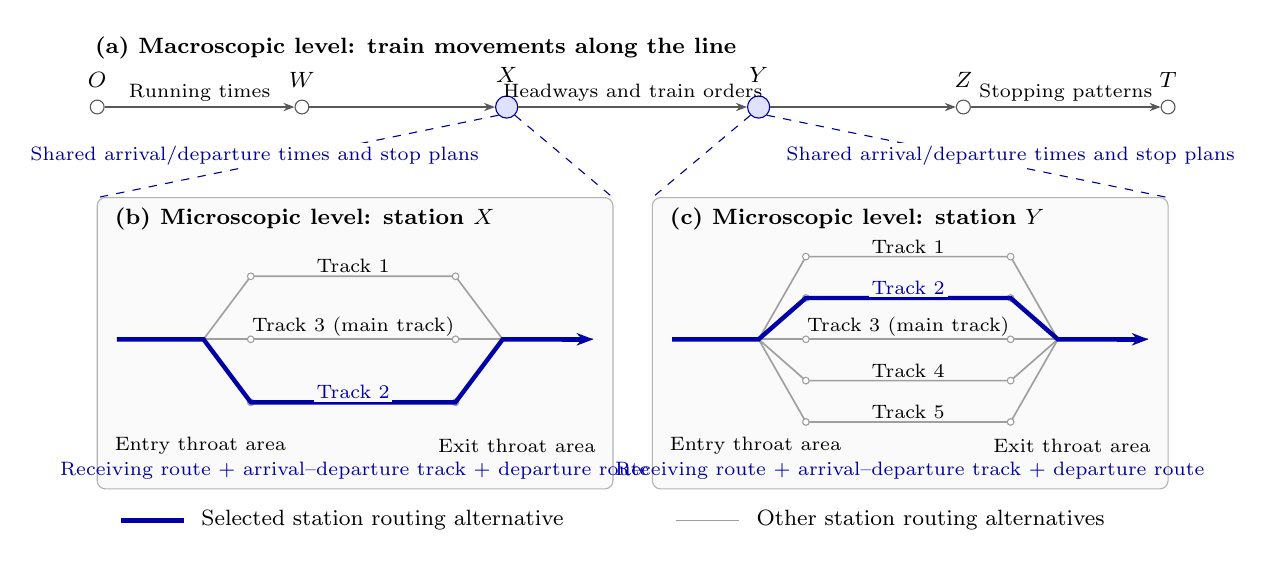
\begin{tikzpicture}[x=1cm,y=1cm,font=\footnotesize,
  stn/.style={circle,draw=gray!70!black,fill=white,inner sep=0pt,minimum size=5pt},
  hub/.style={circle,draw=blue!60!black,fill=blue!12,inner sep=0pt,minimum size=8pt},
  sec/.style={-{Stealth[length=4pt]},gray!70!black,line width=0.5pt},
  trk/.style={gray!75,line width=0.6pt},
  sel/.style={blue!65!black,line width=1.6pt},
  sw/.style={circle,draw=gray!75,fill=white,inner sep=0pt,minimum size=2.4pt},
  tlab/.style={font=\scriptsize,inner sep=1pt,anchor=south}]
% ---------------- (a) macroscopic line
\node[anchor=west,font=\footnotesize\bfseries] at (-0.15,0.75) {(a) Macroscopic level: train movements along the line};
\foreach \n/\x in {O/0,W/2.6,Z/11.0,T/13.6}{\node[stn] (\n) at (\x,0) {}; \node[above=1pt] at (\n.north) {$\n$};}
\node[hub] (X) at (5.2,0) {}; \node[above=1pt] at (X.north) {$X$};
\node[hub] (Y) at (8.4,0) {}; \node[above=1pt] at (Y.north) {$Y$};
\draw[sec] (O)--(W); \draw[sec] (W)--(X); \draw[sec] (X)--(Y); \draw[sec] (Y)--(Z); \draw[sec] (Z)--(T);
\node[tlab] at (1.3,0.03) {Running times};
\node[tlab] at (6.8,0.03) {Headways and train orders};
\node[tlab] at (12.3,0.03) {Stopping patterns};
% ---------------- station boxes and links
\draw[rounded corners=3pt,draw=gray!60,fill=gray!4] (0,-1.15) rectangle (6.55,-4.85);
\draw[rounded corners=3pt,draw=gray!60,fill=gray!4] (7.05,-1.15) rectangle (13.6,-4.85);
\draw[dashed,blue!60!black] (X.south west)--(0,-1.15); \draw[dashed,blue!60!black] (X.south east)--(6.55,-1.15);
\draw[dashed,blue!60!black] (Y.south west)--(7.05,-1.15); \draw[dashed,blue!60!black] (Y.south east)--(13.6,-1.15);
\node[fill=white,inner sep=1pt,text=blue!60!black,font=\scriptsize] at (2.0,-0.62) {Shared arrival/departure times and stop plans};
\node[fill=white,inner sep=1pt,text=blue!60!black,font=\scriptsize] at (11.6,-0.62) {Shared arrival/departure times and stop plans};
\node[anchor=west,font=\footnotesize\bfseries] at (0.1,-1.42) {(b) Microscopic level: station $X$};
\node[anchor=west,font=\footnotesize\bfseries] at (7.15,-1.42) {(c) Microscopic level: station $Y$};
% ---------------- generic station drawing: #1 x-shift, list of track y/labels, selected track y
\foreach \sx/\tracks/\ysel in {
   0/{-2.15/Track 1,-2.95/Track 3 (main track),-3.75/Track 2},
   7.05/{-1.9/Track 1,-2.425/Track 2,-2.95/Track 3 (main track),-3.475/Track 4,-4.0/Track 5}}{
 \begin{scope}[shift={(\sx,0)}]
  \def\ym{-2.95}
  \foreach \y/\lab in \tracks {
    \draw[trk] (1.35,\ym)--(1.95,\y)--(4.55,\y)--(5.15,\ym);
    \node[sw] at (1.95,\y) {}; \node[sw] at (4.55,\y) {};
    \node[tlab] at (3.25,\y) {\lab};}
  \draw[trk] (0.25,\ym)--(1.35,\ym); \draw[trk] (5.15,\ym)--(6.3,\ym);
  \node[anchor=west,font=\scriptsize] at (0.1,-4.3) {Entry throat area};
  \node[anchor=east,font=\scriptsize] at (6.45,-4.3) {Exit throat area};
  \node[text=blue!65!black,font=\scriptsize] at (3.27,-4.62) {Receiving route + arrival--departure track + departure route};
 \end{scope}}
% selected alternatives
\draw[sel] (0.25,-2.95)--(1.35,-2.95)--(1.95,-3.75)--(4.55,-3.75)--(5.15,-2.95)--(6.0,-2.95);
\draw[sel,-{Stealth[length=6pt]}] (5.9,-2.95)--(6.3,-2.95);
\draw[sel] (7.3,-2.95)--(8.4,-2.95)--(9.0,-2.425)--(11.6,-2.425)--(12.2,-2.95)--(13.05,-2.95);
\draw[sel,-{Stealth[length=6pt]}] (12.95,-2.95)--(13.35,-2.95);
\node[tlab,text=blue!65!black,fill=gray!4] at (3.25,-3.75) {Track 2};
\node[tlab,text=blue!65!black,fill=gray!4] at (10.3,-2.425) {Track 2};
% ---------------- legend
\draw[sel] (0.3,-5.25)--(1.1,-5.25); \node[anchor=west] at (1.2,-5.25) {Selected station routing alternative};
\draw[trk] (7.35,-5.25)--(8.15,-5.25); \node[anchor=west] at (8.25,-5.25) {Other station routing alternatives};
\end{tikzpicture}
}
\caption{Illustrative railway line and station track layouts. Blue paths mark the selected station routing alternatives, which are linked to the line by shared arrival and departure times and stop plans.}\label{fig:network}
\end{figure}

A feasible timetable satisfies two levels of constraints. At the macroscopic level, it satisfies the arrival and departure time windows, running and dwell times, minimum headways, train orders, overtaking rules, maintenance windows, maximum travel times, and service frequency requirements. Train stop-count constraints bound the number of stops of a train over a designated route segment, and station service frequency constraints bound the number of stopping trains of a given type at a station within a given service-counting window. A change in arrival or departure time can therefore alter the counted service even if the stopping pattern remains unchanged. At the microscopic level, every train operation is assigned a station routing alternative such that track occupations do not overlap and route headways are respected. The timetable is jointly feasible, i.e., conflict-free at both levels, if both levels are satisfied by the same arrival and departure times, stopping patterns, and station routings.

The objective is lexicographic. The primary objective minimizes the timetable makespan, i.e., the time between the earliest origin departure and the latest destination arrival over all trains. Minimizing the makespan compresses the prescribed services into the shortest operating period while respecting the service frequency requirements and travel time limits. The secondary objectives minimize the weighted deviation from preferred departure and arrival windows and, finally, the total running time supplement.

\subsection{Event-activity network representation}\label{sec:ean}
We represent the problem on an event-activity network, extending the event-based representation of timetables \citep{Serafini1989,Liebchen2007} with the disjunctive activities used for scheduling with shared resources \citep{Bartusch1988,Mascis2002}. Each node is an \emph{event}: the departure of a train at its origin, its arrival at its destination, or its arrival or departure at an intermediate station. Two virtual events $T^-$ and $T^+$ mark the start and the end of the operating period, and a time-origin event $o$ with $t_o=0$ carries absolute time bounds. Each arc $(e,f)$ is an \emph{activity} with a lower bound $l_{ef}$ on its duration, i.e., $t_f-t_e\ge l_{ef}$; an upper bound $t_f-t_e\le u_{ef}$ is represented by the reverse arc $(f,e)$ with $l_{fe}=-u_{ef}$. The activity types are as follows.
\begin{itemize}
\item \emph{Running activities} link the departure at one station with the arrival at the next station of the same train. Their duration lies between the pure running time plus acceleration and deceleration times, which depend on whether the train stops at the two stations, and the same value plus the maximum running time supplement.
\item \emph{Dwell activities} link the arrival and the departure of an intermediate operation. Their duration is zero for a pass; for a stop, it lies between the minimum dwell time and the normal maximum, or the waiting maximum if the train is overtaken.
\item \emph{Section headway activities} link the departures (and the arrivals) of two trains that use the same directed section. They form disjunctive pairs, one for each possible train order; the same order is selected at both ends of a section, so that overtaking can only take place at stations. The minimum headway depends on whether each train stops or passes.
\item \emph{Track occupation activities} link the end of the occupation of one operation with the start of the occupation of another operation at the same station. They exist only if both operations select the same track, and they form a disjunctive pair.
\item \emph{Route headway activities} link the arrival or departure events of two trains at the same station whose selected routes are subject to a route headway. They exist only if the corresponding routes are selected, and they also form disjunctive pairs.
\item \emph{Window activities} link the time origin $o$ with events and represent the arrival and departure time windows, the maintenance windows (traversal before or after the closure), and the position of a stop relative to a service-counting window (before, within, or after it).
\item \emph{Travel time activities} bound the time between the start and the end of a designated journey of a train, and \emph{makespan activities} link $T^-$ with every origin departure and every destination arrival with $T^+$.
\end{itemize}

\Cref{fig:ean}(a) shows the network for two trains $i$ and $j$ running from station $v_1$ to $v_3$ via $v_2$. The running and dwell activities of each train form a chain; the section headway pairs (blue) and the track occupation and route headway pairs at $v_2$ (orange) are disjunctive, and the latter are conditional on the station routing decisions. The discrete decisions of the problem therefore determine \emph{which} activities exist and \emph{how long} they are: the stopping decisions determine the running and dwell bounds and the minimum headways; the train orders select one activity of each section headway pair; the station routings activate track occupation and route headway pairs, of which the orders select one; and the window classifications select one window activity per counted stop. \Cref{fig:ean}(b) shows the network after such a selection, in which train $j$ overtakes train $i$ at $v_2$ while $i$ dwells longer. Once a selection is made, the event times only need to satisfy the remaining difference constraints, and the timetable makespan is determined by the longest chain of tight activities from $T^-$ to $T^+$ (\cref{prop:longest}).

\begin{figure}[tbp]
\centering
\resizebox{\textwidth}{!}{% Event-activity network of two trains i, j on stations v1 -> v2 -> v3 (TikZ)
\newcommand{\eanbase}[1]{%
  % #1 = 1: full network; 2: selected network with critical path
  \begin{tikzpicture}[x=1cm,y=1cm,font=\footnotesize,
    ev/.style={circle,draw=black!80,fill=white,inner sep=0pt,minimum size=17pt,font=\scriptsize},
    vv/.style={rectangle,rounded corners=2pt,draw=black!70,fill=gray!12,inner sep=2pt,minimum size=14pt,font=\scriptsize},
    run/.style={-{Stealth[length=4pt]},line width=0.7pt,black!80},
    dwl/.style={-{Stealth[length=4pt]},line width=0.7pt,black!80,densely dashdotted},
    hw/.style={{Stealth[length=4pt]}-{Stealth[length=4pt]},line width=0.6pt,blue!65!black,dashed},
    hws/.style={-{Stealth[length=4pt]},line width=0.7pt,blue!65!black},
    stn/.style={{Stealth[length=4pt]}-{Stealth[length=4pt]},line width=0.6pt,orange!80!black,dotted},
    stns/.style={-{Stealth[length=4pt]},line width=0.7pt,orange!80!black},
    vir/.style={-{Stealth[length=4pt]},line width=0.5pt,gray},
    crit/.style={line width=2.2pt,red!70!black,opacity=0.35}]
    % station columns
    \foreach \x/\lab in {0/$v_1$,3.6/$v_2$,7.2/$v_3$}{\node[font=\footnotesize\bfseries,gray] at (\x+0.6,3.05) {\lab};}
    \draw[gray!40,rounded corners=3pt] (2.95,-0.55) rectangle (5.45,2.5);
    \node[gray,font=\scriptsize,anchor=north] at (4.2,-0.55) {station $v_2$ (overtaking allowed)};
    % events
    \node[ev] (di1) at (0.6,2) {$d_i^{1}$};  \node[ev] (dj1) at (0.6,0) {$d_j^{1}$};
    \node[ev] (ai2) at (3.4,2) {$a_i^{2}$};  \node[ev] (aj2) at (3.4,0) {$a_j^{2}$};
    \node[ev] (di2) at (5.0,2) {$d_i^{2}$};  \node[ev] (dj2) at (5.0,0) {$d_j^{2}$};
    \node[ev] (ai3) at (7.8,2) {$a_i^{3}$};  \node[ev] (aj3) at (7.8,0) {$a_j^{3}$};
    \node[vv] (Tm) at (-1.3,1) {$T^-$}; \node[vv] (Tp) at (9.7,1) {$T^+$};
    \node[gray,font=\scriptsize,anchor=east] at (-0.15,2) {train $i$};
    \node[gray,font=\scriptsize,anchor=east] at (-0.15,0) {train $j$};
    \ifnum#1=1
      % train activities
      \draw[run] (di1)--node[above,font=\scriptsize]{running} (ai2); \draw[dwl] (ai2)--node[above,font=\scriptsize]{dwell} (di2); \draw[run] (di2)--node[above,font=\scriptsize]{running} (ai3);
      \draw[run] (dj1)--(aj2); \draw[dwl] (aj2)--(dj2); \draw[run] (dj2)--(aj3);
      % disjunctive headway pairs (one order variable per section)
      \draw[hw] (di1)--node[left,font=\scriptsize,blue!65!black]{$z_{ijc_1}$} (dj1);
      \draw[hw] (ai2) to[bend right=18] node[left,font=\scriptsize,blue!65!black,pos=0.3]{$z_{ijc_1}$} (aj2);
      \draw[hw] (di2) to[bend left=18] node[right,font=\scriptsize,blue!65!black,pos=0.3]{$z_{ijc_2}$} (dj2);
      \draw[hw] (ai3)--node[right,font=\scriptsize,blue!65!black]{$z_{ijc_2}$} (aj3);
      % conditional station activities at v2 (track occupancy / route headway)
      \draw[stn] (di2) to[bend left=6] (aj2);
      \draw[stn] (dj2) to[bend left=6] (ai2);
      \node[orange!80!black,font=\scriptsize,align=center,fill=white,inner sep=1pt] at (4.2,1.0) {$w^T,w^{\sigma\sigma'}$\\[-1pt]$\mid Y$};
      % virtual makespan events
      \foreach \e in {di1,dj1}{\draw[vir] (Tm)--(\e);}
      \foreach \e in {ai3,aj3}{\draw[vir] (\e)--(Tp);}
    \else
      % selected network: i first on c1; j overtakes i at v2 (j first on c2); different tracks, route headway active
      \draw[crit] (Tm.east)--(di1.west); \draw[crit] (di1)--(dj1); \draw[crit] (dj1)--(aj2); \draw[crit] (aj2)--(dj2);
      \draw[crit] (dj2)--(di2); \draw[crit] (di2)--(ai3); \draw[crit] (ai3.east)--(Tp.west);
      \draw[run] (di1)--(ai2); \draw[dwl] (ai2)--(di2); \draw[run] (di2)--(ai3);
      \node[font=\scriptsize,anchor=south] at (4.2,2.04) {$\eta_i=1$};
      \draw[run] (dj1)--(aj2); \draw[dwl] (aj2)--(dj2); \draw[run] (dj2)--(aj3);
      \draw[hws] (di1)--node[left,font=\scriptsize,blue!65!black]{$h$} (dj1);
      \draw[hws] (ai2) to[bend right=18] (aj2);
      \draw[hws] (dj2) to[bend right=18] node[right,font=\scriptsize,blue!65!black,pos=0.6]{$h$} (di2);
      \draw[hws] (aj3)--(ai3);
      \draw[stns] (ai2) to[bend left=10] (aj2.north east);
      \node[font=\scriptsize,text=orange!80!black,anchor=west] at (3.75,1.0) {$h_{\rho\rho'}$};
      \foreach \e in {di1,dj1}{\draw[vir] (Tm)--(\e);}
      \foreach \e in {ai3,aj3}{\draw[vir] (\e)--(Tp);}
      \node[red!70!black,font=\scriptsize,anchor=north] at (4.2,-0.95) {critical path: length $=S$ (Proposition~\ref{prop:longest})};
    \fi
  \end{tikzpicture}}
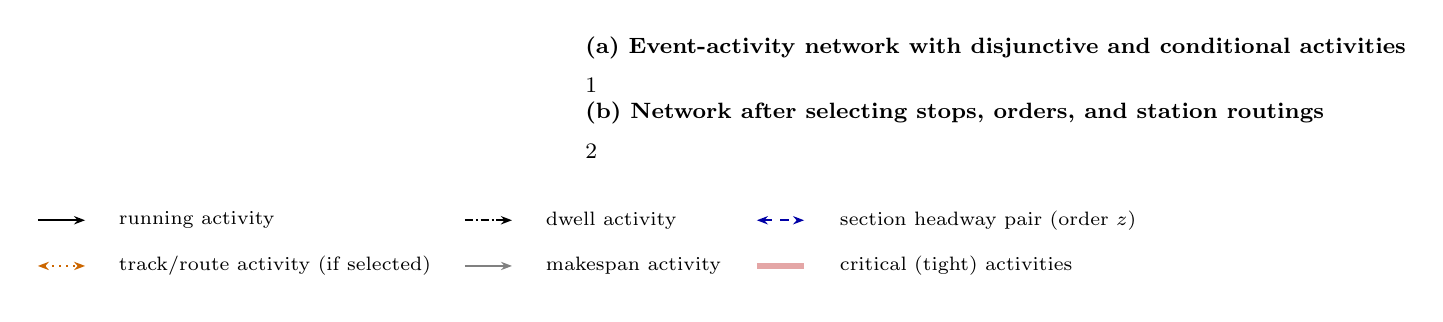
\begin{tikzpicture}[font=\footnotesize]
  \node (a) at (0,0) {\eanbase{1}};
  \node[anchor=north] (b) at ([yshift=-4mm]a.south) {\eanbase{2}};
  \node[anchor=south west,font=\footnotesize\bfseries] at (a.north west) {(a) Event-activity network with disjunctive and conditional activities};
  \node[anchor=south west,font=\footnotesize\bfseries] at (b.north west) {(b) Network after selecting stops, orders, and station routings};
  % legend
  \matrix[anchor=north,below=3mm of b,column sep=3mm,row sep=1mm,font=\scriptsize,
          nodes={anchor=west}] {
    \draw[-{Stealth[length=4pt]},line width=0.7pt] (0,0)--(0.6,0); & \node{running activity}; &
    \draw[-{Stealth[length=4pt]},line width=0.7pt,densely dashdotted] (0,0)--(0.6,0); & \node{dwell activity}; &
    \draw[{Stealth[length=4pt]}-{Stealth[length=4pt]},line width=0.6pt,blue!65!black,dashed] (0,0)--(0.6,0); & \node{section headway pair (order $z$)}; \\
    \draw[{Stealth[length=4pt]}-{Stealth[length=4pt]},line width=0.6pt,orange!80!black,dotted] (0,0)--(0.6,0); & \node{track/route activity (if selected)}; &
    \draw[-{Stealth[length=4pt]},line width=0.5pt,gray] (0,0)--(0.6,0); & \node{makespan activity}; &
    \draw[line width=2.2pt,red!70!black,opacity=0.35] (0,0)--(0.6,0); & \node{critical (tight) activities}; \\
  };
\end{tikzpicture}
}
\caption{Event-activity network for two trains $i$ and $j$ travelling from $v_1$ to $v_3$. (a) Running and dwell activities form one chain per train; section headway pairs are selected by the train order $z$ (one order per section), and track occupation and route headway pairs exist only for the selected station routings $Y$. (b) After the selection ($i$ before $j$ on $c_1$; $j$ overtakes $i$ at $v_2$; different tracks with an active route headway), the shaded critical path determines the timetable makespan.}\label{fig:ean}
\end{figure}

The representation is used in three ways. First, the mathematical formulation in \cref{sec:model} is organized by activity type, so that every constraint corresponds to one type of arc in \cref{fig:ean}. Second, the conflicts diagnosed by the algorithm are violated activities: macroscopic conflicts are violated running, dwell, section headway, window, or travel time activities, and station conflicts are violated track occupation or route headway activities. Third, for a fixed selection, the activities with zero slack identify the decisions that must change to reduce the makespan; the quality search of the algorithm builds its neighborhoods from these activities (\cref{sec:joint}).

\subsection{Interdependence of stop planning, timetabling, and platforming}
\Cref{fig:exchange} illustrates how a coordinated stop exchange can resolve a track conflict at station $X$ while maintaining the service frequencies. Train $B$ cannot stop at $X$ without overlapping the occupations of trains $A$ and $C$, and the main track cannot accommodate a stop. Exchanging the stops of trains $B$ and $D$ between stations $X$ and $Y$ preserves the displayed train and station counts, but the revised times and station routings still require feasibility checks. Even if a stop is retained, moving its reference event across a service-counting window boundary can change the station count. A compensating stop on another train must respect its stop-count limits, other service frequency requirements, and station track and route constraints. On the event-activity network, the exchange removes the dwell and track occupation activities of $B$ at $X$, adds those of $D$, changes the running activities and minimum headways of both trains, and may change the selected window activities. These dependencies require coordinated changes to stops, arrival and departure times, and station routings, with affected counts remaining within their prescribed bounds.

\begin{figure}[tb]
\centering
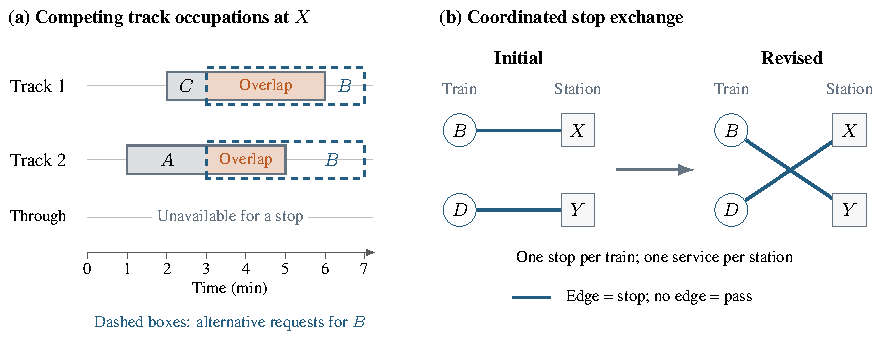
\includegraphics[width=0.85\textwidth]{figures/fig2_stop_exchange.pdf}
\caption{Illustrative stop exchange: (a) competing track occupations at station $X$; (b) revised stops preserving the displayed train and station service frequencies.}\label{fig:exchange}
\end{figure}

\subsection{Assumptions}
The following assumptions are made throughout the paper.
\begin{enumerate}[label=(A\arabic*)]
\item The train services, their station sequences, and their train types are prescribed, and no train can be cancelled. Rolling stock circulation, passenger assignment, and infrastructure changes are not considered.
\item Train operations in the two directions do not interfere with each other. Overtaking is only possible at stations where it is allowed, and a stopping train can be overtaken by at most one other train at a station. A dwell time longer than the normal maximum is permitted only for such waiting and is subject to a separate upper bound.
\item The timetable is non-periodic and covers one operating day, with arrival and departure times on a continuous time scale.
\item An intermediate stop occupies its track from arrival to departure, whereas a pass and the departure (arrival) at an origin (destination) occupy the track only at the instant of departure (arrival); no additional time is reserved for train preparation or stabling. The separation between movements of different trains in a station is represented by route headways.
\item Maintenance windows are given; each window closes a directed section during a fixed period.
\end{enumerate}

\section{Mathematical formulation}\label{sec:model}
The formulation follows the activity types of \cref{sec:ean}. It links train movements and station routings through shared arrival and departure times and stop decisions. All times, durations, headways, and big-$M$ coefficients are in seconds.

\subsection{Notation}
\Cref{tab:notation} summarizes the notation. At each station, a train has at most one operation, which is either a stop or a pass. An operation $n=(i,v)\in\Nset$ represents train $i$ stopping at or passing through station $v$; the train associated with operation $n$ is denoted by $i(n)$, and $\Nset_v$ contains the operations at station $v$. Consecutive operations $n$ and $n^+$ of the same train define a running arc $\ell=(n,n^+)\in\Aset$ on a directed section $c\in\Cset$. The event set $\Eset$ comprises the departures at origins, the arrivals at destinations, and the arrivals and departures at intermediate stations; $t_e$ denotes the time of event $e$, and $a_n$ and $d_n$ denote the arrival and departure times of operation $n$ where these events exist.

The stop--pass status of an operation is denoted by $m\in\{0,1\}$, where $m=1$ denotes a stop and $m=0$ a pass. For operation $n$ with status $m$, $\Rset^m_n$ is the set of station routing alternatives; alternative $r$ specifies the track $k(r)$, the receiving route $\rho^{\mathrm{in}}(r)$, and the departure route $\rho^{\mathrm{out}}(r)$. Alternatives are indexed separately by stop--pass status, even when they use the same track and routes. Let $\Gset_n\subseteq\{\mathrm{in},\mathrm{out}\}$ be the set of route types required by operation $n$, where ``in'' denotes the receiving route and ``out'' the departure route: $\Gset_n=\{\mathrm{out}\}$ at an origin, $\{\mathrm{in}\}$ at a destination, and $\{\mathrm{in},\mathrm{out}\}$ at an intermediate station. The hard event bounds $[L_e,U_e]$, derived from the given arrival and departure time windows, apply to every timetable and remain valid for all admissible stopping and ordering decisions. They differ from the preferred event windows $[\lb{W}_e,\ub{W}_e]$, whose violations contribute to $P$, and from the service-counting windows $[A_q,B_q]$, which determine the stops counted by station rules. For a conditional constraint $f\ge h$, the big-$M$ coefficient is set to $M=\max\{0,h-L_f\}$, where $L_f$ is a valid lower bound of $f$ and $h$ the largest applicable value; a tilde denotes the coefficient of the reverse order.

\begin{table}[tbp]
\centering\small
\caption{Notation.}\label{tab:notation}
\setlength{\tabcolsep}{4pt}
\renewcommand{\arraystretch}{1.08}
\begin{tabular}{@{}>{$}l<{$}>{\raggedright\arraybackslash}p{120mm}@{}}\toprule
\multicolumn{2}{@{}l}{\textit{Sets and indices}}\\
\Iset,\Vset,\Cset & Trains $i,j$; stations $v$; directed sections $c$\\
\Nset,\Nset_v & Train operations $n=(i,v)$; operations at station $v$\\
\Nset^{o},\Nset^{d},\Nset^{\mathrm{int}} & Origin, destination, and intermediate operations\\
\Aset & Running arcs $\ell=(n,n^+)$ of consecutive operations of a train\\
\Eset,\Eset^W & Events $e$ (arrivals and departures); events with a preferred window\\
\Rset^m_n,\Rset_n & Station routing alternatives $r$ of operation $n$ with status $m$; $\Rset_n=\Rset^0_n\cup\Rset^1_n$\\
\Gset_n & Route types (``in'': receiving, ``out'': departure) required by operation $n$\\
\Qset^{\mathrm{tr}},\Qset^{\mathrm{st}} & Train stop-count rules; station service frequency rules $q$\\
\Qset^{J},\Qset^{M} & Maximum travel time rules; maintenance windows\\
\Nset_q & Operations counted by rule $q$\\
\Bset_n & Overtaking indicators $b_{ijv}$ of intermediate operation $n=(i,v)$\\
\multicolumn{2}{@{}l}{\textit{Parameters}}\\
L_e,U_e & Hard lower and upper bounds of the time of event $e$\\
r_\ell,\alpha_\ell,\beta_\ell & Pure running time; additional acceleration and deceleration times of arc $\ell$\\
\bar u_\ell & Maximum running time supplement of arc $\ell$\\
\delta_n,\bar\delta^N_n,\bar\delta^W_n & Minimum, normal maximum, and waiting maximum dwell times of operation $n$\\
h^{\vartheta,mm'}_{ijc} & Minimum headway on section $c$ at its departure ($\vartheta=D$) or arrival ($\vartheta=A$) end for stop--pass statuses $(m,m')$\\
h_{\rho\rho'} & Route headway from route $\rho$ to route $\rho'$\\
\lb{K}_q,\ub{K}_q & Minimum and maximum number of counted stops of rule $q$\\
{[A_q,B_q]} & Service-counting window of station rule $q$\\
T^{\max}_q & Maximum travel time of rule $q$\\
{[A^M_q,B^M_q]} & Closure period of maintenance window $q$\\
{[\lb{W}_e,\ub{W}_e]},\omega^\pm_e & Preferred window of event $e$; early and late weights\\
\multicolumn{2}{@{}l}{\textit{Decision variables}}\\
a_n,d_n,t_e & Arrival time, departure time; time of event $e$\\
s_n\in\{0,1\} & 1 if operation $n$ is a stop, 0 if a pass\\
u_\ell\ge0 & Running time supplement of arc $\ell$\\
z_{ijc}\in\{0,1\} & Train order on section $c$: 0 if train $i$ precedes train $j$\\
b_{ijv},\eta_n\in[0,1] & Train $j$ overtakes train $i$ at station $v$; operation $n$ is overtaken\\
\xi_{\ell q}\in\{0,1\} & 1 if arc $\ell$ is traversed before maintenance window $q$, 0 if after\\
c_{nq},\lambda^-_{nq},\lambda^+_{nq}\in\{0,1\} & Stop of operation $n$ within, before, or after the window of rule $q$\\
y_{nr}\in\{0,1\} & 1 if operation $n$ uses station routing alternative $r$\\
Y^{T}_{nk},Y^{\sigma}_{n\rho} & 1 if operation $n$ uses track $k$; route $\rho$ on side $\sigma\in\Gset_n$\\
w^{T}_{nn'},w^{\sigma\sigma'}_{nn'}\in\{0,1\} & Track and route-event order: 1 if operation $n$ precedes $n'$\\
S,P,R\ge0 & Timetable makespan, preferred-window deviation penalty, total supplement\\\bottomrule
\end{tabular}
\end{table}

\subsection{Objective function}
Let $o_i$ and $f_i$ be the origin and destination operations of train $i$. With auxiliary variables $T^-,T^+\in\mathbb{R}$ (the times of the virtual events) and $p^-_e,p^+_e\ge0$,
\begin{equation}
T^-\le d_{o_i},\quad T^+\ge a_{f_i}\quad(i\in\Iset),\qquad S=T^+-T^-,\label{eq:span}
\end{equation}
\begin{equation}
p^-_e\ge\lb{W}_e-t_e,\quad p^+_e\ge t_e-\ub{W}_e\quad(e\in\Eset^W),\qquad P=\sum_{e\in\Eset^W}(\omega^-_ep^-_e+\omega^+_ep^+_e),\qquad R=\sum_{\ell\in\Aset}u_\ell.\label{eq:pr}
\end{equation}
The objective lexicographically minimizes $(S,P,R)$, where $S$ denotes the timetable makespan, $P$ the weighted deviation from the preferred event windows, and $R$ the total running time supplement. Constraints \eqref{eq:span} are the makespan activities of the network. The secondary objectives distinguish timetables with equal makespans; $P$ favours timetables close to the preferred departure and arrival times, and $R$ avoids unnecessary supplements.

\subsection{Running, dwell, window, and travel time activities}
\textbf{Event time windows and stop decisions.} Train times must remain within the prescribed event bounds, and stopping decisions must respect mandatory stops and passes. The bounds $\lb{s}_n,\ub{s}_n$ also enforce stops at origins and destinations and exclude stop--pass statuses without admissible station routing alternatives:
\begin{equation}
L_e\le t_e\le U_e\quad(e\in\Eset),\qquad \lb{s}_n\le s_n\le\ub{s}_n,\quad s_n\in\{0,1\}\quad(n\in\Nset).\label{eq:bounds}
\end{equation}
\textbf{Running and dwell activities.} On arc $\ell=(n,n^+)$, the running time comprises the pure running time, the acceleration and deceleration additions of the stops at both ends, and a bounded supplement. At an intermediate station, the dwell time of a stop lies between the minimum and the normal maximum; the waiting maximum applies only when the train is overtaken ($\eta_n=1$, \cref{sec:headway}). A pass has zero dwell:
\begin{equation}
a_{n^+}-d_n=r_\ell+\alpha_\ell s_n+\beta_\ell s_{n^+}+u_\ell,\qquad 0\le u_\ell\le\bar u_\ell\qquad(\ell\in\Aset),\label{eq:run}
\end{equation}
\begin{equation}
\delta_ns_n\le d_n-a_n\le\bar\delta^N_ns_n+(\bar\delta^W_n-\bar\delta^N_n)\eta_n,\qquad 0\le\eta_n\le s_n\qquad(n\in\Nset^{\mathrm{int}}).\label{eq:dwell}
\end{equation}
\textbf{Travel time and maintenance window activities.} Rule $q\in\Qset^J$ bounds the travel time from the starting operation $n^o_q$ to the ending operation $n^d_q$, including intermediate dwell. For maintenance window $q\in\Qset^M$, arc $\ell=(n,n^+)$ is unavailable during $[A^M_q,B^M_q]$; the binary indicator $\xi_{\ell q}$ selects traversal before the closure ($\xi_{\ell q}=1$) or after it ($\xi_{\ell q}=0$), and $M^{\mathrm{b}}_{\ell q}$, $M^{\mathrm{a}}_{\ell q}$ are valid coefficients:
\begin{equation}
a_{n^d_q}-d_{n^o_q}\le T^{\max}_q\quad(q\in\Qset^J),\qquad a_{n^+}\le A^M_q+M^{\mathrm{b}}_{\ell q}(1-\xi_{\ell q}),\ \ d_n\ge B^M_q-M^{\mathrm{a}}_{\ell q}\xi_{\ell q}\ \ (q\in\Qset^M).\label{eq:maint}
\end{equation}

\subsection{Service frequency constraints}
Stopping decisions must satisfy train stop-count and station service requirements. Rule $q\in\Qset^{\mathrm{tr}}$ bounds the number of stops over a prescribed route segment, counting its endpoints only when specified. Rule $q\in\Qset^{\mathrm{st}}$ bounds the number of stopping trains of a given type at a station within the closed window $[A_q,B_q]$. For station service rules, the reference time is $\theta_n=d_n$ at origins and $\theta_n=a_n$ otherwise. The indicator $c_{nq}$ equals one when operation $n$ stops and its reference time lies in the closed window:
\begin{equation}
\begin{gathered}
\lb{K}_q\le\sum_{n\in\Nset_q}s_n\le\ub{K}_q\qquad(q\in\Qset^{\mathrm{tr}}),\\
c_{nq}=s_n\,\mathbf{1}_{[A_q,B_q]}(\theta_n)\ \ (n\in\Nset_q),\qquad \lb{K}_q\le\sum_{n\in\Nset_q}c_{nq}\le\ub{K}_q\qquad(q\in\Qset^{\mathrm{st}}).
\end{gathered}\label{eq:freq}
\end{equation}
Both window endpoints count, passes contribute zero, and overlapping windows are evaluated independently.

\textbf{Window classification.} To generate candidates with a MILP, the exact counting rule in \eqref{eq:freq} is relaxed by classifying each eligible stop as before, within, or after the window. These classifications are the window activities of the network. The binary variables $\lambda^-_{nq}$ and $\lambda^+_{nq}$ indicate a stop of operation $n$ before or after the window, respectively, with $M^Q_{nq}=\max\{0,B_q-L_{\theta_n},U_{\theta_n}-A_q\}$:
\begin{equation}
\begin{gathered}
\lambda^-_{nq}+c_{nq}+\lambda^+_{nq}=s_n,\qquad
A_q-M^Q_{nq}(1-c_{nq})\le\theta_n\le B_q+M^Q_{nq}(1-c_{nq}),\\
\theta_n\le A_q+M^Q_{nq}(1-\lambda^-_{nq}),\qquad
\theta_n\ge B_q-M^Q_{nq}(1-\lambda^+_{nq})\qquad(q\in\Qset^{\mathrm{st}},\ n\in\Nset_q).
\end{gathered}\label{eq:freqlin}
\end{equation}
If train $i(n)$ passes the station, all three indicators are zero. Since a MILP cannot represent the strict inequalities $\theta_n<A_q$ and $\theta_n>B_q$, constraints \eqref{eq:freqlin} also allow a stop exactly at a window endpoint to be classified as outside the window. Constraints \eqref{eq:freqlin} thus provide a MILP relaxation of the exact closed-window counting rule \eqref{eq:freq}. Every candidate generated with \eqref{eq:freqlin} is recounted under \eqref{eq:freq} before acceptance (\cref{sec:accept}).

\subsection{Section headway, train order, and overtaking constraints}\label{sec:headway}
Trains sharing a section require minimum separation, which varies with their stop--pass statuses. For operations $n,n'$ of different trains, $h^{mm'}\ge0$ is the minimum headway for statuses $(m,m')$, and $q_{nn'}\in[0,1]$ represents $s_ns_{n'}$. For trains $(i,j)$ sharing directed section $c$, $t^D_{ic}$ and $t^A_{ic}$ denote the upstream departure and the downstream arrival. The status-dependent headway $H(s_n,s_{n'})$ is
\begin{equation}
\begin{gathered}
q_{nn'}\le s_n,\qquad q_{nn'}\le s_{n'},\qquad q_{nn'}\ge s_n+s_{n'}-1,\\
H(s_n,s_{n'})=h^{00}+(h^{10}-h^{00})s_n+(h^{01}-h^{00})s_{n'}+(h^{11}-h^{10}-h^{01}+h^{00})q_{nn'}.
\end{gathered}\label{eq:hw}
\end{equation}
The disjunctive pair of section headway activities is selected by one train order $z_{ijc}$, which applies at both ends of the section and thus excludes overtaking within sections:
\begin{equation}
t^\vartheta_{jc}-t^\vartheta_{ic}\ge H^\vartheta_{ijc}(s)-M^\vartheta_{ijc}z_{ijc},\qquad
t^\vartheta_{ic}-t^\vartheta_{jc}\ge H^\vartheta_{jic}(s)-\tilde M^\vartheta_{ijc}(1-z_{ijc})\qquad(\vartheta\in\{D,A\}),\label{eq:order}
\end{equation}
where $M^\vartheta_{ijc}=\max\{0,\max_{m,m'}h^{\vartheta,mm'}_{ijc}+U_{t^\vartheta_{ic}}-L_{t^\vartheta_{jc}}\}$. Analogous constraints with binary order variables $z^V_{ef}\in\{0,1\}$ separate the arrival and departure events $(e,f)$ of different trains at station $v$ for which a station headway is specified. The minimum headways in \eqref{eq:hw}--\eqref{eq:order} are derived from the route headways as the smallest separation over all admissible route combinations for the given stop--pass statuses, so they are necessary conditions for station feasibility. Imposing a larger value at the macroscopic level would exclude feasible uses of less restrictive routes; the headways of the routes actually selected are imposed in \cref{sec:platforming}.

\textbf{Overtaking.} Station overtaking links a change in train order to an extended dwell. For trains $i$ and $j$ sharing the incoming and outgoing sections $c^-$ and $c^+$ of station $v$, we set $z_{ijc^-}=z_{ijc^+}$ where overtaking is prohibited. Otherwise, $b_{ijv}$ indicates that $j$ overtakes $i$ at $v$, with $i$ ahead on $c^-$ and behind on $c^+$. For an intermediate operation $n=(i,v)$, $\Bset_n$ contains the indicators $b_{ijv}$ of the trains $j$ that may overtake train $i$ at $v$, and $b$ denotes an element of $\Bset_n$. The indicator $\eta_n$ equals one if train $i$ is overtaken at $v$:
\begin{equation}
\begin{gathered}
b_{ijv}\le1-z_{ijc^-},\qquad b_{ijv}\le z_{ijc^+},\qquad b_{ijv}\ge z_{ijc^+}-z_{ijc^-},\\
\eta_n\ge b\ \ (b\in\Bset_n),\qquad \eta_n\le\textstyle\sum_{b\in\Bset_n}b\le1\qquad(n\in\Nset^{\mathrm{int}}).
\end{gathered}\label{eq:overtake}
\end{equation}
Because the order variables are binary, $b_{ijv}$ takes integer values without being declared binary. The last inequality permits at most one overtaking train per stop, and together with \eqref{eq:dwell} a dwell beyond the normal maximum is only possible if the train is actually overtaken; $\eta_n=0$ if $\Bset_n=\emptyset$.

\subsection{Train platforming constraints}\label{sec:platforming}
\textbf{Station routing selection.} Each operation must use a compatible combination of track and routes for its stop--pass status. The model selects one alternative consistent with the stop decision and derives the resource-use indicators: $Y^T_{nk}$ equals one when operation $n$ occupies track $k$, and $Y^\sigma_{n\rho}$ when it uses route $\rho$ on side $\sigma\in\Gset_n$:
\begin{equation}
\sum_{r\in\Rset_n}y_{nr}=1,\quad\sum_{r\in\Rset^1_n}y_{nr}=s_n,\quad
Y^T_{nk}=\sum_{r\in\Rset_n:k(r)=k}y_{nr},\quad Y^\sigma_{n\rho}=\sum_{r\in\Rset_n:\rho^\sigma(r)=\rho}y_{nr}\ \ (\sigma\in\Gset_n).\label{eq:select}
\end{equation}
\textbf{Track occupation activities.} Operations assigned to the same track must have non-overlapping occupations. The occupation interval $[B_n,E_n]$ is $[d_n,d_n]$ at an origin, $[a_n,a_n]$ at a destination, and $[a_n,d_n]$ at an intermediate station. For $n,n'\in\Nset_v$ with $i(n)\ne i(n')$ and any common admissible track $k$, the binary order $w^T_{nn'}$ selects one activity of the disjunctive pair when both operations select $k$:
\begin{equation}
B_{n'}-E_n\ge-M^T_{nn'}(3-w^T_{nn'}-Y^T_{nk}-Y^T_{n'k}),\qquad
B_n-E_{n'}\ge-\tilde M^T_{nn'}(2+w^T_{nn'}-Y^T_{nk}-Y^T_{n'k}),\label{eq:track}
\end{equation}
with, e.g., $M^T_{nn'}=\max\{0,U_{E_n}-L_{B_{n'}}\}$. A pass occupies the point $a_n=d_n$, which cannot lie strictly inside the occupation of another train; contact at the boundary remains subject to the route headways.

\textbf{Route headway activities.} Different trains may conflict on routes through the station throat even when they use different tracks. Let $\tau^{\mathrm{in}}_n=a_n$ and $\tau^{\mathrm{out}}_n=d_n$. For $n,n'\in\Nset_v$ with $i(n)\ne i(n')$, sides $\sigma\in\Gset_n$ and $\sigma'\in\Gset_{n'}$, and applicable routes $(\rho,\rho')$, the binary order $w^{\sigma\sigma'}_{nn'}$ selects the event order on which the route headway is imposed:
\begin{equation}
\begin{gathered}
\tau^{\sigma'}_{n'}-\tau^\sigma_n\ge h_{\rho\rho'}-M^{\sigma\sigma'}_{nn'\rho\rho'}(3-w^{\sigma\sigma'}_{nn'}-Y^\sigma_{n\rho}-Y^{\sigma'}_{n'\rho'}),\\
\tau^\sigma_n-\tau^{\sigma'}_{n'}\ge h_{\rho'\rho}-\tilde M^{\sigma\sigma'}_{nn'\rho\rho'}(2+w^{\sigma\sigma'}_{nn'}-Y^\sigma_{n\rho}-Y^{\sigma'}_{n'\rho'}).
\end{gathered}\label{eq:route}
\end{equation}
Route pairs with a headway in at least one direction are included, with zero for a missing direction; this covers identical routes ($\rho=\rho'$) and movements on different tracks. The receiving and departure routes of the same operation must be compatible but are not separated by a headway. Only the selected resources activate \eqref{eq:track}--\eqref{eq:route}.

\subsection{Integrated model and structural properties}\label{sec:integrated}
Let $x$ collect the times, stops, train orders, window and maintenance classifications, and auxiliary variables. Set $X^M$ imposes \eqref{eq:span}--\eqref{eq:overtake} with the exact counting rule \eqref{eq:freq}, and $Y_v(x)$ contains the routing selections and orders at station $v$ satisfying \eqref{eq:select}--\eqref{eq:route}. Together they define the integrated model and its jointly feasible set:
\begin{equation}
\begin{gathered}
\operatorname{lexmin}\,(S,P,R)\quad\text{s.t.}\quad x\in X^M,\quad (y_v,w_v)\in Y_v(x)\ \ (v\in\Vset),\\
X^{\mathrm{joint}}=\{x\in X^M:Y_v(x)\ne\emptyset\ \text{for all}\ v\in\Vset\}.
\end{gathered}\label{eq:model}
\end{equation}
Replacing \eqref{eq:freq} with \eqref{eq:freqlin} gives the MILP used to generate candidates; its solutions must be recounted under \eqref{eq:freq} before acceptance. We call the vector $\pi=(s,z,z^V,\eta,\xi,c,\lambda,y,w)$ of all discrete decisions the \emph{structure} of a timetable.

\begin{proposition}[Station decomposition]\label{prop:decomp}
For fixed event times and stop decisions $x$, the constraints \eqref{eq:select}--\eqref{eq:route} decompose into independent station platforming problems, one for each $v\in\Vset$, and $x\in X^{\mathrm{joint}}$ if and only if each of them is feasible.
\end{proposition}
\begin{proof}
For fixed $x$, the variables $y_{nr}$, $Y$, and $w$ of operations at station $v$ only appear in constraints \eqref{eq:select}--\eqref{eq:route} written for pairs $n,n'\in\Nset_v$. No constraint links variables of different stations, so the feasibility problem separates by station.
\end{proof}

\begin{proposition}[Makespan of a fixed structure]\label{prop:longest}
Let $\pi$ be a structure, and let $G(\pi)$ be the network obtained from the event-activity network by keeping, for each disjunctive pair, the activity selected by $\pi$ and by setting all activity lengths according to $\pi$. If the system of event times consistent with $\pi$ is feasible, then the minimum makespan $S^*(\pi)$ subject to \eqref{eq:span}--\eqref{eq:route} with $\pi$ fixed equals the length of a longest path from $T^-$ to $T^+$ in $G(\pi)$. Moreover, the system is feasible if and only if $G(\pi)$ contains no cycle of positive length.
\end{proposition}
\begin{proof}
With $\pi$ fixed, every constraint in \eqref{eq:span}--\eqref{eq:route} reduces to a difference constraint $t_f-t_e\ge l_{ef}$ between two event times, or to a bound $L\le t_e\le U$, which is the difference constraint with the time-origin event $o$, $t_o=0$. This holds for the running activities \eqref{eq:run} after eliminating $u_\ell\in[0,\bar u_\ell]$ (two difference constraints), the dwell activities \eqref{eq:dwell}, the travel time and maintenance activities \eqref{eq:maint}, the window classifications \eqref{eq:freqlin}, the selected section headways \eqref{eq:order}, and the active track occupation and route headway activities \eqref{eq:track}--\eqref{eq:route}; the inactive ones are redundant by the choice of the big-$M$ coefficients. A system of difference constraints is feasible if and only if its constraint graph has no positive cycle, and the minimum of $t_{T^+}-t_{T^-}$ is the length of a longest $T^-$--$T^+$ path, which follows from linear programming duality (the dual is a unit-flow problem from $T^-$ to $T^+$) and is the classical result for project networks with minimum and maximum time lags \citep{Bartusch1988}.
\end{proof}

\Cref{prop:longest} has two consequences that are used by the algorithm. First, for a fixed structure, the timetable can be re-optimized by a linear program in which all event times move together; we use this in the fixed-structure re-optimization of \cref{sec:accept}. Second, the makespan of a structure can only be reduced by changing a decision that affects every longest path, i.e., the stop, order, routing, or window classification associated with at least one critical activity. The quality search therefore starts its neighborhoods from the trains that determine the earliest departure and the latest arrival and from chains of tight activities (\cref{sec:joint}).

\begin{remark}[Model size and complexity]\label{rem:size}
The platforming subproblem alone is NP-complete when each train has three or more routing possibilities \citep{Kroon1997}. In the integrated model, the numbers of order variables $w$ and of constraints \eqref{eq:track}--\eqref{eq:route} grow quadratically with the number of operations per station and linearly with the number of route pairs with a headway. \Cref{tab:size} in \cref{sec:cases} reports the sizes of the full MILP for the test cases, which reach about $1.4\times10^7$ constraints and $7.0\times10^5$ binary variables in the large-scale case.
\end{remark}

\section{Conflict-driven adaptive large neighborhood search}\label{sec:alg}
Model \eqref{eq:model} becomes difficult to solve directly as the numbers of trains and stations grow. We therefore develop a CD-ALNS. Unlike classical ALNS for timetabling, which removes and reinserts trains by heuristic rules \citep[e.g.,][]{Dong2020}, each destroy operator of the CD-ALNS releases a conflict-related subset of stop, event time, train order, and platforming decisions, and the repair step re-optimizes them by solving a restricted MILP with a commercial solver while the remaining decisions are fixed. The method is thus a MILP-based neighborhood search \citep{Fischetti2003,Danna2005} whose neighborhoods are defined on the event-activity network and adapted by the ALNS mechanism of \citet{Ropke2006}.

\subsection{Algorithm framework}\label{sec:framework}
The algorithm has three phases (\cref{fig:framework} and \cref{alg:cdalns}): macroscopic timetable construction (Phase 1), joint feasibility search (Phase 2), and joint quality search (Phase 3). In each iteration, conflict information determines the decisions to be reconsidered, adaptive selection chooses a destroy operator and a neighborhood size, and the restricted MILP determines the revised decisions. Each phase keeps its own operator weights. Three solutions are distinguished: the \emph{current solution}, from which neighborhoods are built; a pool of \emph{working candidates}, which are completely evaluated but may still contain conflicts; and the \emph{best jointly feasible timetable}, which is only replaced by a strictly better jointly feasible timetable. All steps, including model construction, solution, and feasibility checks, share one time limit. The failure or timeout of a restricted repair does not prove infeasibility of the original problem; it only triggers the selection of another operator or a larger neighborhood.

\begin{figure}[tb]
\centering
\resizebox{\textwidth}{!}{% Figure 3: framework of the conflict-driven ALNS (TikZ)
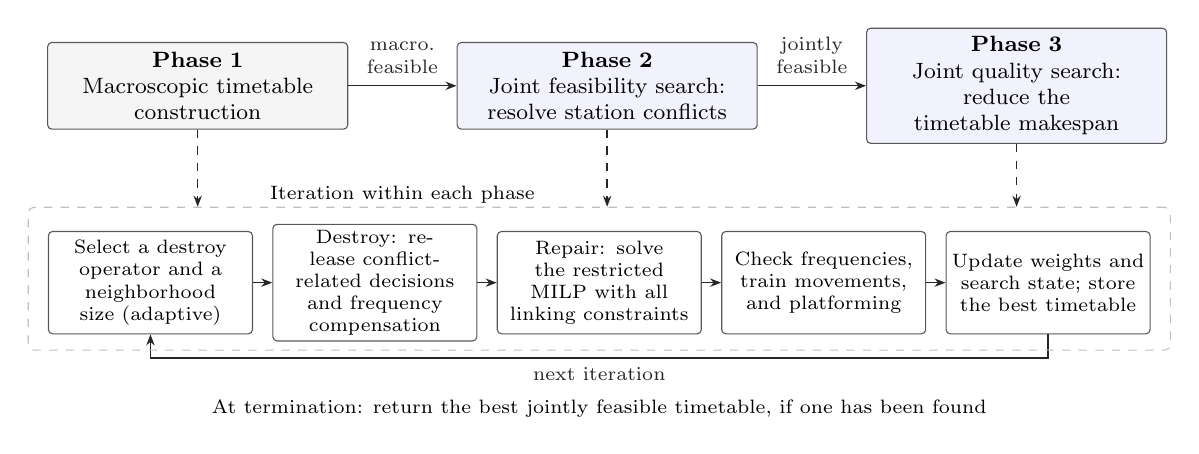
\begin{tikzpicture}[font=\footnotesize,
  phase/.style={draw=gray!70!black,rounded corners=1.5pt,align=center,inner sep=3pt,text width=36mm,minimum height=11mm,fill=blue!5},
  stp/.style={draw=gray!70!black,rounded corners=1.5pt,align=center,inner sep=2pt,text width=24.5mm,minimum height=13mm,fill=white,font=\scriptsize},
  arr/.style={-{Stealth[length=4pt]},gray!30!black,line width=0.5pt}]
% phases
\node[phase,fill=gray!8] (p1) at (0,0) {\textbf{Phase 1}\\Macroscopic timetable\\construction};
\node[phase] (p2) at (52mm,0) {\textbf{Phase 2}\\Joint feasibility search:\\resolve station conflicts};
\node[phase] (p3) at (104mm,0) {\textbf{Phase 3}\\Joint quality search:\\reduce the timetable makespan};
\draw[arr] (p1) -- node[above=1pt,font=\scriptsize,align=center]{macro.\\feasible} (p2);
\draw[arr] (p2) -- node[above=1pt,font=\scriptsize,align=center]{jointly\\feasible} (p3);
% iteration loop shared by all phases
\node[stp] (s1) at (-6mm,-25mm) {Select a destroy operator and a neighborhood size (adaptive)};
\node[stp] (s2) at (22.5mm,-25mm) {Destroy: release conflict-related decisions and frequency compensation};
\node[stp] (s3) at (51mm,-25mm) {Repair: solve the restricted MILP with all linking constraints};
\node[stp] (s4) at (79.5mm,-25mm) {Check frequencies, train movements, and platforming};
\node[stp] (s5) at (108mm,-25mm) {Update weights and search state; store the best timetable};
\foreach \a/\b in {s1/s2,s2/s3,s3/s4,s4/s5}{\draw[arr] (\a) -- (\b);}
\draw[arr] (s5.south) -- ++(0,-3mm) -| node[pos=0.25,below,font=\scriptsize]{next iteration} (s1.south);
\node[draw=gray!50,dashed,rounded corners=2pt,fit=(s1)(s5),inner sep=2.5mm,yshift=0.5mm] (loop) {};
\node[anchor=south,font=\scriptsize,fill=white,inner sep=1pt] at (26mm,0 |- loop.north) {Iteration within each phase};
\draw[arr,dashed] (p1.south) -- (p1.south |- loop.north);
\draw[arr,dashed] (p2.south) -- (p2.south |- loop.north);
\draw[arr,dashed] (p3.south) -- (p3.south |- loop.north);
\node[anchor=north,font=\scriptsize,align=center] at ([yshift=-5mm]loop.south) {At termination: return the best jointly feasible timetable, if one has been found};
\end{tikzpicture}
}
\caption{Framework of the CD-ALNS. Each phase repeats the destroy-and-repair iteration with its own adaptive weights.}\label{fig:framework}
\end{figure}

\begin{algorithm}[tbp]
\caption{Conflict-driven adaptive large neighborhood search (CD-ALNS)}\label{alg:cdalns}
\small
\begin{algorithmic}[1]
\Require instance data; time limit $\Theta$; operator sets $\mathcal{O}^M=\{M1,\dots,M4\}$, $\mathcal{O}^J=\{J1,\dots,J5\}$; three scales
\Ensure best jointly feasible timetable $x^\star$, or the status that none was found
\State $x^\star\gets\emptyset$; initialize the weights $w^M,w^F,w^Q$ of all operator--scale pairs to one
\State construct a stopping pattern satisfying \eqref{eq:freq} under provisional times; solve a sparse macroscopic MILP $\to x$ \Comment{\cref{sec:init}}
\While{$x$ violates a macroscopic constraint \textbf{and} time remains} \Comment{Phase 1}
  \State diagnose the violated activities of $x$; select $(o,\kappa)\in\mathcal{O}^M\times\{1,2,3\}$ by \eqref{eq:select-prob} with $w^M$
  \State release the decisions defined by $(o,\kappa)$ and the compensation set (\cref{alg:nbh}); solve the restricted macroscopic MILP $\to x'$
  \State if $x'$ improves the diagnostic score, $x\gets x'$; reward $(o,\kappa)$ and update $w^M$ by \eqref{eq:weights}
\EndWhile
\State assign station routings to $x$ station by station (\cref{prop:decomp}), allowing elastic slacks $\to$ working pool $\mathcal{W}$
\While{time remains}
  \If{$x^\star=\emptyset$} \Comment{Phase 2}
    \State take an anchor $x$ from $\mathcal{W}$; seeds $\gets$ operations in track or route conflicts of $x$; weights $w\gets w^F$; ranking $\Phi\gets\Phi^F$
  \Else \Comment{Phase 3}
    \State take $x$ as the current quality solution; seeds $\gets$ trains defining $T^-$ and $T^+$ in $x$; $w\gets w^Q$; $\Phi\gets\Phi^Q$
    \State occasionally apply fixed-structure re-optimization to $x^\star$ (\cref{sec:accept})
  \EndIf
  \State select $(o,\kappa)\in\mathcal{O}^J\times\{1,2,3\}$ by \eqref{eq:select-prob} with $w$, skipping duplicates and suspended pairs
  \State build the neighborhood $\mathcal{F}$ from the seeds by \cref{alg:nbh}; solve the restricted MILP over $\mathcal{F}$ $\to x'$ \Comment{\cref{sec:repair}}
  \State recount service frequencies under \eqref{eq:freq}; correct window misclassifications if necessary
  \State evaluate $x'$ completely; if $x'$ has no unresolved station, insert it into $\mathcal{W}$ ranked by $\Phi$
  \If{$x'$ passes all macroscopic and microscopic checks \textbf{and} $\Phi^Q(x')\prec\Phi^Q(x^\star)$}
    \State $x^\star\gets x'$ \Comment{\cref{sec:accept}}
  \EndIf
  \State update the current solution by the acceptance rule; reward $(o,\kappa)$ and update $w$ by \eqref{eq:weights}; update stagnation counters
\EndWhile
\State \Return $x^\star$
\end{algorithmic}
\end{algorithm}

\subsection{Initialization and macroscopic timetable construction}\label{sec:init}
\textbf{Initial candidate.} Initialization first selects a stopping pattern that satisfies the train stop-count bounds and the station service frequency requirements under provisional event times. These times establish service-count compatibility but do not yet constitute a feasible timetable. A reduced macroscopic MILP then imposes all train-level activities (running, dwell, window, and travel time activities) and a selected set of inter-train relations, namely the section headway pairs of train pairs that are close in time. Inter-train relations that are omitted from the reduced model are not dropped from the problem: complete macroscopic checks evaluate all of them, and relations found violated are added to the model in later repairs. The candidate generator may keep several candidates and returns the best according to the diagnostic score below.

\textbf{Macroscopic diagnosis.} The complete macroscopic check evaluates every activity in \eqref{eq:bounds}--\eqref{eq:overtake}. It reports the violated train pairs and operations and computes the weighted diagnostic score
\begin{equation}
D(x)=\Delta^{H}(x)+180\,n^{O}(x)+600\,n^{W}(x)+600\,n^{Q}(x),\label{eq:diag}
\end{equation}
where $\Delta^H$ is the total headway deficit in seconds, $n^O$ the number of other order and overtaking violations, $n^W$ the number of long dwells without an actual overtaking, and $n^Q$ the total violation of service frequency bounds. $D$ ranks candidates and determines rewards; it is not a feasibility certificate, and only a candidate with all macroscopic activities satisfied proceeds to the joint search.

\textbf{Macroscopic operators.} Conflict diagnosis identifies the train pairs and operations around which the four macroscopic operators in \cref{tab:operators} act:
\begin{itemize}
\item \textbf{M1 Time} adjusts arrival and departure times and supplements in \eqref{eq:run}--\eqref{eq:dwell} within a time radius to remove headway deficits in \eqref{eq:order}, without changing stops or orders.
\item \textbf{M2 Order--time} additionally permits re-sequencing selected conflicting train pairs, consistently with \eqref{eq:order}--\eqref{eq:overtake}; on the network, it re-selects the section headway activity of these pairs.
\item \textbf{M3 Waiting support} acts only on long dwells without overtaking. Releasing the orders on the sections before and after the station permits either an actual overtaking or a shorter dwell under \eqref{eq:dwell} and \eqref{eq:overtake}. It is not applicable when no such dwell exists.
\item \textbf{M4 Stop--frequency} permits optional stop changes under \eqref{eq:bounds} and \eqref{eq:freq} for the trains involved in conflicts or frequency violations, together with the service frequency compensation of \cref{alg:nbh} and the related orders and times.
\end{itemize}
The three scales of every macroscopic operator limit the restricted model to at most 160, 320, or 640 train pairs and the movement of event times to 600, 1200, or 2400~s; M4 may change at most 6, 12, or 18 stops. All section constraints, including those linking released and fixed decisions, are retained, and headway violations are represented by nonnegative slacks during Phase~1. When restricted repairs fail or repeatedly time out, the scale is enlarged. After three iterations without improvement, the search alternates one iteration of a rule-based bounded repair with three adaptive iterations; rewards obtained by the rule-based fallback are not credited to any operator.

\subsection{Joint neighborhoods with service frequency compensation}\label{sec:joint}
\textbf{Seeds and expansion.} In the joint feasibility phase, neighborhoods are built around the train operations involved in track occupation or route headway conflicts, i.e., violated station activities. Conflicts are taken in decreasing order of violation, together with other conflicts at the same or adjacent stations within about 600~s. In the quality phase, the seeds are the trains that determine the earliest origin departure and the latest destination arrival in \eqref{eq:span}, including ties, i.e., the start and end of the critical paths of \cref{prop:longest}. In both phases, the seeds are expanded to the operations of the same trains at neighboring stations, to the trains that use the same stations at close times, and to the operations needed for service frequency compensation. The three scales allow at most 12, 20, or 32 trains and 4, 8, or 12 stop changes, with a time radius of 600~s, 1800~s, or no radius, and the expansion covers 2, 4, or all neighboring stations of each seed train.

\textbf{Joint operators.} Five joint operators are used in Phases 2 and 3:
\begin{itemize}
\item \textbf{J1 Joint} coordinates stops, orders, times, and routings throughout the neighborhood, coupling the service counts in \eqref{eq:freq} with the station activities \eqref{eq:select}--\eqref{eq:route}. It is the most flexible operator and handles general station conflicts.
\item \textbf{J2 Time} retains the stops and all section orders in \eqref{eq:order} and releases the event times; the station routings at the affected stations are re-optimized. It resolves conflicts that can be removed by shifting arrival and departure times combined with a change of track or route, without changing the stopping pattern.
\item \textbf{J3 Service frequency} starts from J1 and adds the stopping and timing decisions identified through the affected service-count constraints by \cref{alg:nbh}. At the three scales it may include up to 32, 48, or 64 operations of 12, 20, or 32 trains. Train orders and station routings remain jointly adjustable within the resulting neighborhood.
\item \textbf{J4 Boundary} adds up to 2, 4, or 6 trains outside the J1 neighborhood that interact with the selected trains through the section headway, track occupation, or route headway activities \eqref{eq:order}, \eqref{eq:track}, and \eqref{eq:route} and have the highest conflict pressure across the boundary. At the largest scale, their operations along the entire route are released.
\item \textbf{J5 Tight temporal links} expands J1 along chains of tight or nearly tight activities under the current stopping and routing decisions, i.e., running, dwell, train order, track occupation, and route headway activities with (almost) zero slack. The associated decisions are reconsidered jointly with any required service frequency compensation. J5 is activated after three iterations without improvement in the feasibility search; in the quality search, it releases the train orders and station routings on the critical activities that block further makespan reduction (\cref{prop:longest}).
\end{itemize}
Neighborhoods that release the same decisions with the same time ranges and stop-change limits are considered only once, so that renaming an operator does not increase its selection probability. A neighborhood that has failed for the same anchor is suspended for 4, 8, 16, and then 32 iterations; when all applicable neighborhoods are suspended, the one tried least recently is used.

\textbf{Service frequency compensation.} For the current count $C_q=\sum_{n\in\Nset_q}c_{nq}$ of a station rule, the admissible count change is
\begin{equation}
\lb{K}_q-C_q\ \le\ \Delta C_q\ \le\ \ub{K}_q-C_q.\label{eq:comp}
\end{equation}
Stop changes and time shifts across counting-window boundaries can alter $C_q$. For a given set of released decisions, \cref{alg:nbh} computes the smallest and largest counts that the released decisions could produce. If the smallest count could fall below $\lb{K}_q$, operations that can add a counted stop are included: an optional stop of another train inside the window, or an existing stop whose time can move into the window. Symmetrically, if the largest count could exceed $\ub{K}_q$, operations that can remove a counted stop are included. Candidates are chosen by their remaining room under their own stop-count rules and by their time distance to the window, and the expansion is bounded by the scale limits. For example, losing a counted stop at a rule's lower bound requires another stop within that window; the compensating train must also respect its own stop-count limits, the bounds of other affected service counts, and the station track and route constraints. The restricted MILP determines these changes jointly; counts need not retain their previous values if they remain within their bounds. Train stop-count rules are treated in the same way.

\begin{algorithm}[tbp]
\caption{Neighborhood construction with service frequency compensation}\label{alg:nbh}
\small
\begin{algorithmic}[1]
\Require current solution $x$; seeds; operator $o$; scale limits (trains, stop changes, time radius)
\Ensure released decisions $\mathcal{F}$ (stops, event times, orders, station routings)
\State $\mathcal{F}\gets$ decisions of the seed operations permitted by $o$; expand along the seed trains and to trains at the same stations at close times
\If{$o\in\{\mathrm{J4}\}$} add the trains outside $\mathcal{F}$ with the highest boundary conflict pressure \EndIf
\If{$o\in\{\mathrm{J5}\}$} add the decisions on chains of tight activities starting from the seeds \EndIf
\Repeat
  \For{each train stop-count or station rule $q$ that contains a released operation}
    \State compute the minimum and maximum counts $\lb{C}_q(\mathcal{F})$, $\ub{C}_q(\mathcal{F})$ attainable by changing only the decisions in $\mathcal{F}$
    \If{$\lb{C}_q(\mathcal{F})<\lb{K}_q$} add operations that can add a counted stop (optional stop or time shift into the window) \EndIf
    \If{$\ub{C}_q(\mathcal{F})>\ub{K}_q$} add operations that can remove a counted stop \EndIf
  \EndFor
\Until{no rule is added \textbf{or} a scale limit is reached}
\State add the station routings of all trains at the stations affected by $\mathcal{F}$ (background trains keep their times)
\State \Return $\mathcal{F}$
\end{algorithmic}
\end{algorithm}

\subsection{Restricted MILP repair}\label{sec:repair}
The restricted MILP is constructed from the complete macroscopic model. Decisions outside the neighborhood are fixed to their values in the anchor solution, released event times may move within the intersection of their hard bounds and the time radius, and running time supplements may change only on arcs with at least one released end. All constraints that involve a released decision are retained, including those that link it to fixed decisions; the model is compiled by eliminating fixed variables rather than by deleting constraints. At every station affected by the neighborhood, station routing variables and order variables are built for all operations at that station, including background trains whose times are fixed, so that a released train can be accommodated by re-routing other trains.

Before the first jointly feasible timetable is found, nonnegative slacks relax the track occupation and route headway constraints \eqref{eq:track}--\eqref{eq:route}. Candidates are ranked by $\Phi^F=(V^{\mathrm{micro}},P,S,R)$, where $V^{\mathrm{micro}}$ sums the temporal separation deficits in seconds under the evaluated resource assignment. For each unordered pair of station operations and each applicable track or route-event relation, the smaller nonnegative deficit over the two precedence orders is used; scores are summed over relations and pairs, and a microscopic conflict is a pair with a positive score. This diagnostic measures neither the total overlap duration nor the timetable extension needed for feasibility. After station conflict reduction, $P$ precedes $S$ to favour timetables close to the preferred windows during feasibility restoration. The quality search requires zero slack and uses the objective order of the problem, $\Phi^Q=(S,P,R)$. Auxiliary terms, such as the number of stop changes and the total movement of event times, may be added with low priority to stabilize the repair. Window-endpoint misclassifications under \eqref{eq:freqlin} are corrected locally by linking the affected in-window indicator to the stop decision or, if necessary, by re-solving the complete macroscopic model; the reward of such a recovery is not credited to the original operator. The restricted model is not built if it would exceed 2\,000\,000 station constraints or 200\,000 integer variables; the attempt is then recorded as unsuccessful.

\subsection{Adaptive operator selection}\label{sec:adaptive}
Following \citet{Ropke2006}, each pair $a$ of operator and scale in the applicable set $\Aset^{\mathrm{act}}$ is selected with probability
\begin{equation}
p_a=(1-\epsilon)\frac{w_a}{\sum_{b\in\Aset^{\mathrm{act}}}w_b}+\frac{\epsilon}{|\Aset^{\mathrm{act}}|},\label{eq:select-prob}
\end{equation}
where $w_a$ is the current weight and $\epsilon$ controls uniform exploration. Separate weights are kept for the macroscopic, joint feasibility, and joint quality phases, so that success in removing violations is not taken as evidence that the same operator will compress a feasible timetable. For $N_a>0$ observations of $a$ in an observation period, with rewards $r_k\ge0$ and computation times $\tau_k>0$, the weights are updated as
\begin{equation}
\begin{gathered}
w^+_a=\max\{w_{\min},(1-\lambda)w_a+\lambda g_a\},\qquad
g^M_a=\frac{\sum_{k:a_k=a}r_k}{N_a},\\ g^F_a=\frac{\sum_{k:a_k=a}r_k}{\sum_{k:a_k=a}\tau_k/\tau_0},\qquad
g^Q_a=\frac{\bar r_a}{\min\{2,\max\{0.5,\sqrt{\bar\tau_a/\tau_0}\}\}},
\end{gathered}\label{eq:weights}
\end{equation}
where $g^M_a$, $g^F_a$, and $g^Q_a$ are the scores in the three phases, $\bar r_a$ and $\bar\tau_a$ are the average reward and computation time, and the square root moderates the time penalty in the quality phase. Pairs not used in a period keep their weights. The rewards are listed in \cref{tab:params}: the first macroscopically or jointly feasible timetable receives 8, a new best diagnostic score or solution 4, and another improvement 1; the joint rewards add the normalized improvement of the first differing component of $\Phi$; a secondary improvement at equal makespan receives 0.1, and an unvisited accepted structure 0.05 in the quality phase. Invalid candidates receive zero. In the quality phase, the time limit of each repair is also selected adaptively among 60, 180, and 600~s.

\begin{table}[tb]
\centering\small
\caption{Destroy operators of the CD-ALNS.}\label{tab:operators}
\setlength{\tabcolsep}{4pt}
\begin{tabular}{@{}>{\raggedright\arraybackslash}p{27mm}>{\raggedright\arraybackslash}p{38mm}>{\raggedright\arraybackslash}p{34mm}>{\raggedright\arraybackslash}p{50mm}@{}}\toprule
Operator & Released decisions & Fixed decisions & Typical conflict addressed\\\midrule
\multicolumn{4}{@{}l}{\textit{Macroscopic operators (Phase 1)}}\\
M1 Time & Event times, supplements & Stops, all train orders & Headway deficits that small time shifts can remove\\
M2 Order--time & Times, orders of selected train pairs & Stops & Conflicts that require re-sequencing two trains\\
M3 Waiting support & Orders on adjacent sections, times & Stops & Long dwells without an overtaking train\\
M4 Stop--frequency & Optional stops, related orders, times & Other stops & Frequency violations; conflicts caused by stops\\\midrule
\multicolumn{4}{@{}l}{\textit{Joint operators (Phases 2 and 3)}}\\
J1 Joint & Stops, orders, times, routings & Decisions outside the neighborhood & General station conflicts\\
J2 Time & Times, routings & Stops, all train orders & Conflicts solvable by time shifts and re-routing\\
J3 Service frequency & J1 with service frequency compensation & Decisions outside the neighborhood & Conflict repairs affecting service counts\\
J4 Boundary & J1 plus extra trains & Remaining trains & Conflicts propagating across the boundary\\
J5 Tight temporal links & Decisions along tight activities & Other decisions & Running, dwell, order, track, and route restrictions; critical activities\\\bottomrule
\end{tabular}
\end{table}

\begin{table}[tb]
\centering\small
\caption{Parameters of the CD-ALNS used in all experiments.}\label{tab:params}
\setlength{\tabcolsep}{4pt}
\begin{tabular}{@{}>{\raggedright\arraybackslash}p{70mm}>{\raggedright\arraybackslash}p{78mm}@{}}\toprule
Parameter & Value\\\midrule
Exploration rate $\epsilon$; smoothing $\lambda$; minimum weight $w_{\min}$ & 0.15; 0.25; 0.05\\
Initial weights; observation period; reference time $\tau_0$ & 1; 10 observations; 60 s\\
Rewards (first feasible / new best / improvement) & 8 / 4 / 1 (+ normalized gain in Phases 2--3)\\
Quality rewards (secondary improvement / diversity) & 0.1 / 0.05\\
Macroscopic scales: train pairs; time radius; stop changes (M4) & 160/320/640; 600/1200/2400 s; 6/12/18\\
Joint scales: trains; stop changes; time radius; neighbor stations & 12/20/32; 4/8/12; 600 s/1800 s/none; 2/4/all\\
J3 limits (operations); J4 extra trains & 32/48/64; 2/4/6\\
Suspension of failed neighborhoods & 4, 8, 16, 32 iterations\\
Quality repair time limits & 60, 180, 600 s (selected adaptively)\\
Acceptance threshold (quality phase) & $\min\{30\ \mathrm{s},0.0025S^\star\}\times$ remaining time fraction\\
Restricted MILP size limits & $2\times10^6$ station constraints; $2\times10^5$ integer variables\\\bottomrule
\end{tabular}
\end{table}

\subsection{Solution acceptance and fixed-structure timetable re-optimization}\label{sec:accept}
\textbf{Acceptance.} A candidate is accepted as jointly feasible only if it satisfies all macroscopic activities, including the exact service counts under \eqref{eq:freq}, and if an independent check confirms that its station routings satisfy \eqref{eq:select}--\eqref{eq:route} at every station. The accepted timetable is saved and re-read with the saved tracks and routes fixed, and checked again. Jointly feasible timetables are compared lexicographically by $(S,P,R)$, computed from the continuous event times, with absolute differences of at most $10^{-6}$ treated as ties. During stagnation, i.e., after six quality iterations without improvement, the current solution of the quality search may move to an unvisited jointly feasible structure whose makespan exceeds that of the best timetable $S^\star$ by at most $\min\{30\ \mathrm{s},0.0025S^\star\}$, scaled by the remaining fraction of the time limit, provided that its penalty $P$ does not exceed that of the best timetable. This allowance explores alternative stopping patterns, train orders, and station routings, while the best timetable is retained.

\textbf{Fixed-structure re-optimization.} By \cref{prop:longest}, the timetable of a fixed structure can be re-optimized by a linear program. Fixed-structure re-optimization fixes the stops, train orders, maintenance and window classifications, station routings, and track and route precedences of the best timetable and adjusts all event times simultaneously. The resulting linear program minimizes $S$, then $P$, then $R$; each attained value is imposed as an upper bound in the next stage, and a lower-priority stage is only solved after the preceding one is optimal. Before optimization, the source timetable is checked to be feasible for the fixed structure, so that an incorrectly built model cannot exclude it. The re-optimization allows improvements beyond the time radii of the neighborhoods; its optimality concerns only the fixed structure, and J5 can subsequently release orders or routes on critical activities that block further compression. Its computation time is limited to a small share of the remaining time, and the same structure is not re-optimized repeatedly.

\section{Computational experiments}\label{sec:exp}
\subsection{Test cases and experimental settings}\label{sec:cases}
We evaluate the approach on three cases of different scales (\cref{tab:cases}). The small-scale case is a generated line with 5 stations and 30 trains of two types. The medium- and large-scale cases contain 12 stations with 60 trains and 29 stations with 101 trains, respectively, on lines of 172.1 and 1320~km. The cases differ not only in size but also in the density of their constraints: the medium-scale case has 75 station service frequency rules and 1855 route headway records, and the large-scale case has 2929 train operations with 1449 optional stops and 8047 route headway records.

\begin{table}[tb]
\centering\small
\caption{Characteristics of the test cases (computed from the input data).}\label{tab:cases}
\setlength{\tabcolsep}{4pt}
\begin{tabular}{@{}>{\raggedright\arraybackslash}p{78mm}rrr@{}}\toprule
 & Small & Medium & Large\\\midrule
Stations / sections & 5 / 4 & 12 / 11 & 29 / 28\\
Line length (km) & 66.0 & 172.1 & 1320.0\\
Trains / train types & 30 / 2 & 60 / 1 & 101 / 1\\
Train operations at stations & 150 & 685 & 2929\\
\quad mandatory stops / optional / mandatory passes & 62/88/0 & 120/445/120 & 288/1449/1192\\
Station tracks / receiving and departure routes & 16 / 24 & 63 / 173 & 195 / 493\\
Route headway records & 144 & 1855 & 8047\\
Station service frequency rules / train stop-count rules & 6 / 30 & 75 / 60 & 21 / 101\\
Maintenance window records / maximum travel time rules & 8 / 30 & 22 / 1 & 56 / 32\\
Time limit (h) & 1 & 6 & 6\\\bottomrule
\end{tabular}
\end{table}

The CD-ALNS is compared with two benchmarks. \emph{Direct MILP} solves the full MILP \eqref{eq:model} with the window classification \eqref{eq:freqlin} by Gurobi, minimizing $S$, $P$, and $R$ in sequence. \emph{LBBD} adapts the decomposition of \citet{Leutwiler2022} to the operating rules and data considered here: a macroscopic master problem determines times and stops, and station subproblems check platforming and return logical feasibility cuts. Its results therefore describe this adaptation rather than the original implementation. LBBD terminates at its first jointly feasible timetable, whereas CD-ALNS continues to improve the timetable. All solutions are checked against the same original constraints, including the exact service counting \eqref{eq:freq}. \Cref{tab:size} reports the sizes of the full MILP solved by Direct MILP, taken from the solver logs; they illustrate why the full model becomes impractical as the number of operations per station grows.

\begin{table}[tb]
\centering\small
\caption{Size of the full MILP (Gurobi log of Direct MILP, before presolve).}\label{tab:size}
\begin{tabular}{@{}lrrrr@{}}\toprule
Case & Constraints & Variables & Binary variables & Nonzeros\\\midrule
Small-scale & 74\,497 & 11\,009 & 4\,445 & 327\,305\\
Medium-scale & 990\,153 & 159\,979 & 111\,621 & 4\,504\,111\\
Large-scale & 13\,996\,162 & 1\,071\,296 & 701\,533 & 67\,266\,880\\\bottomrule
\end{tabular}
\end{table}

The algorithms are implemented in C\# on .NET 8 and use Gurobi 10.0.1 for all MILP and LP models. All experiments, including the benchmarks and the ablation, were performed on the same hardware with Intel Xeon E7-4850 v4 processors, using four threads. The time limit is one hour for the small-scale case and six hours for the other cases, and every run in this section uses one random seed. The parameters of the CD-ALNS are listed in \cref{tab:params}.

\subsection{Comparison of solution methods}\label{sec:compare}
We compare solution quality using the timetable makespan $S$, the preferred-window deviation penalty $P$, and the total running time supplement $R$ (\cref{tab:results}). Computation times record the first joint feasibility $t_{\mathrm{feas}}$, the first attainment of the best timetable makespan $t_{\mathrm{best}}$, and the total runtime $t_{\mathrm{run}}$. A dash and the status ``No joint solution'' indicate that no jointly feasible timetable was found before termination; this does not prove infeasibility.

\begin{table}[tb]
\centering\small
\caption{Computational results ($S$, $R$, and times in seconds; $P$ in weighted seconds).}\label{tab:results}
\footnotesize\setlength{\tabcolsep}{3.2pt}
\begin{tabular}{@{}llrrrrrrl@{}}\toprule
Case & Method & $S$ & $P$ & $R$ & $t_{\mathrm{feas}}$ & $t_{\mathrm{best}}$ & $t_{\mathrm{run}}$ & Status\\\midrule
Small-scale & CD-ALNS & 11\,385 & 0 & 0 & 10.41 & 76.64 & 3425.94 & Feasible\\
 & Direct MILP & 11\,385 & 0 & 0 & 35.67 & 35.67 & 56.08 & Makespan optimal\\
 & LBBD & 11\,385 & 0 & 0 & 1227.68 & 1227.68 & 1227.68 & Feasible\\\midrule
Medium-scale & CD-ALNS & 54\,525 & 272\,686 & 1926 & 428.89 & 4823.61 & 21\,026.71 & Feasible\\
 & Direct MILP & -- & -- & -- & -- & -- & 21\,007.85 & No joint solution\\
 & LBBD & -- & -- & -- & -- & -- & 21\,014.79 & No joint solution\\\midrule
Large-scale & CD-ALNS & 65\,849 & 3\,910\,668 & 4946 & 5199.39 & 15\,305.02 & 21\,121.28 & Feasible\\
 & Direct MILP & -- & -- & -- & -- & -- & 21\,092.48 & No joint solution\\
 & LBBD & -- & -- & -- & -- & -- & 21\,148.95 & No joint solution\\\bottomrule
\end{tabular}
\end{table}

In the small-scale case, all three methods attain the timetable makespan of 11\,385~s, which Direct MILP proves to be optimal. CD-ALNS finds joint feasibility first; Direct MILP attains the optimum earlier and has the shortest total runtime. For the medium-scale case, CD-ALNS finds joint feasibility at 428.89~s and reduces the timetable makespan from 59\,970 to 54\,525~s (9.08\%). Neither benchmark finds joint feasibility under the six-hour budget: Direct MILP finds no incumbent, and LBBD remains at its first master problem. For the large-scale case, CD-ALNS attains macroscopic and joint feasibility at 2467.08 and 5199.39~s, respectively, and reduces the timetable makespan from 68\,975 to 65\,849~s (4.53\%). Neither benchmark finds a jointly feasible timetable; LBBD completes one master iteration without an incumbent. These outcomes reflect the difficulty of obtaining a feasible master or full-model solution rather than the quality of the Benders cuts. Without valid lower bounds for the medium- and large-scale cases, the CD-ALNS optimality gaps remain unknown.

\subsection{Convergence analysis}\label{sec:convergence}
To examine feasibility restoration, we follow the medium-scale run in \cref{fig:restoration}. Initially, 84 macroscopic diagnostic conditions are violated (78 headway, four section-order, and two overtaking-cap conditions), with 20 long dwells without overtaking counted separately. Round 1 produces no candidate; round 2 reduces the counts to 23 and 4, and round 3 removes both. The macroscopically feasible timetable still contains nine conflicting station-operation pairs with a 2515~s aggregate separation deficit, although all section headways, which are lower bounds on the route headways, are satisfied. Joint repair removes both in nine rounds.

\begin{figure}[tb]
\centering
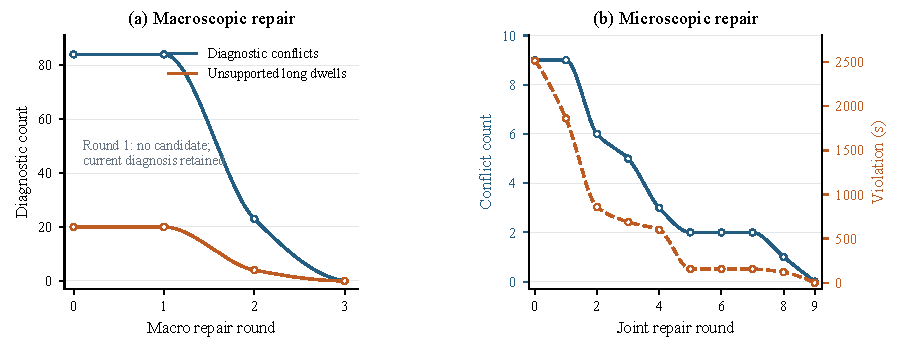
\includegraphics[width=0.86\textwidth]{figures/fig4_restoration.pdf}
\caption{Feasibility restoration in the medium-scale case: (a) violated macroscopic diagnostic conditions and long dwells without overtaking; (b) conflicting station-operation pairs and their aggregate temporal violation score. Round 0 gives the initial diagnosis.}\label{fig:restoration}
\end{figure}

After joint feasibility is reached, the timetable makespan is reduced further (\cref{fig:makespan}). In the small-scale case, the CD-ALNS reaches the optimal timetable makespan after two reductions. In the medium-scale case, the makespan decreases through eight improvements, seven of which occur within the first hour; in the large-scale case it decreases through four improvements. In the large-scale case, the first fixed-structure timetable re-optimization reduces the makespan from 68\,975 to 66\,929~s, i.e., by about two thirds of the total reduction, which illustrates the value of moving all event times of a structure together (\cref{prop:longest}).

\begin{figure}[tb]
\centering
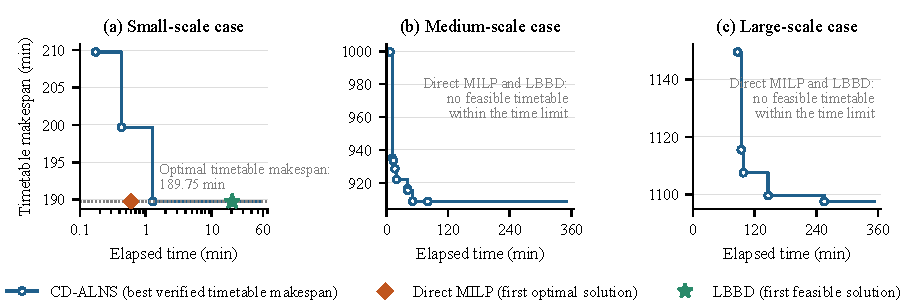
\includegraphics[width=\textwidth]{figures/fig5_makespan.pdf}
\caption{Best verified timetable makespan during optimization. The small-scale case uses a logarithmic time axis; each curve ends at the termination of its run.}\label{fig:makespan}
\end{figure}

\subsection{Analysis of the obtained timetables}\label{sec:solution}
\Cref{fig:solution} shows the best timetable of the medium-scale case and the track occupation at its busiest intermediate station. The 60 trains are accommodated between 06:33 and 21:41:45, i.e., within the makespan of 908.75~min, and overtaking takes place at several intermediate stations, visible as longer horizontal segments of the overtaken trains. Station S3 serves 25 intermediate stops on three tracks; in the period shown in \cref{fig:solution}(b), the stops are spread over two arrival--departure tracks, while passing trains use the main track. The time--distance diagram of the large-scale case is given in \cref{app:large}.

\begin{figure}[tb]
\centering
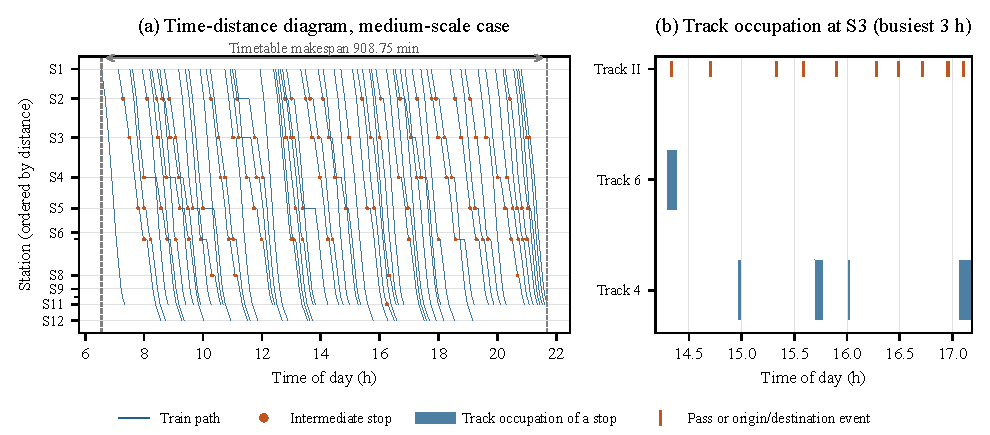
\includegraphics[width=\textwidth]{figures/fig_solution_medium.pdf}
\caption{Best jointly feasible timetable of the medium-scale case: (a) time--distance diagram, with stops marked; (b) track occupation at station S3 in its busiest three-hour period. Stations are numbered along the line.}\label{fig:solution}
\end{figure}

\Cref{tab:solution} summarizes the stopping and resource use of the best timetables, recounted from the saved solutions under the exact rule \eqref{eq:freq}. All service frequency requirements are satisfied, and many of them are binding: in the medium-scale case, 44 of the 75 station rules are exactly at their lower bound, and the average count exceeds the lower bound by only 0.59 stops. Binding service requirements are the situation in which a stop cannot be removed to resolve a conflict without compensation elsewhere, which is what the joint neighborhoods of \cref{sec:joint} provide.

\begin{table}[tb]
\centering\small
\caption{Stopping and station resource use of the best timetables.}\label{tab:solution}
\begin{tabular}{@{}lrrr@{}}\toprule
 & Small & Medium & Large\\\midrule
Intermediate operations / intermediate stops & 90 / 50 & 565 / 113 & 2727 / 707\\
Optional stops: available / used & 88 / 48 & 445 / 113 & 1449 / 621\\
Station service frequency rules & 6 & 75 & 21\\
\quad at lower bound / at upper bound / violated & 6 / 6 / 0 & 44 / 0 / 0 & 5 / 5 / 0\\
\quad average count above lower bound & 0.00 & 0.59 & 20.57\\
Station tracks used / available & 14 / 16 & 31 / 63 & 112 / 195\\\bottomrule
\end{tabular}
\end{table}

\subsection{Effect of the macroscopic ALNS phase}\label{sec:ablation}
To examine the role of the macroscopic ALNS, the ablation replaces it with the rule-based bounded repair of the initialization procedure, retaining the joint ALNS and identical data, objectives, time limit, joint settings, seed, solver, and hardware. In this paired medium-scale run (\cref{fig:ablation}), the full configuration reaches macroscopic and joint feasibility at 128.37 and 428.89~s, versus 2709.69 and 3159.98~s. It also reaches the shared final timetable makespan of 54\,525~s earlier (4823.61 versus 6039.26~s). The ablated configuration has lower final secondary objectives ($P=233\,464$, $R=933$~s, versus 272\,686 and 1926~s); the full configuration therefore does not improve every objective. Its macroscopic phase ends after three rounds, before the first weight update, so this observed improvement precedes adaptive weight learning and stems from the conflict-driven macroscopic operators.

\begin{figure}[tb]
\centering
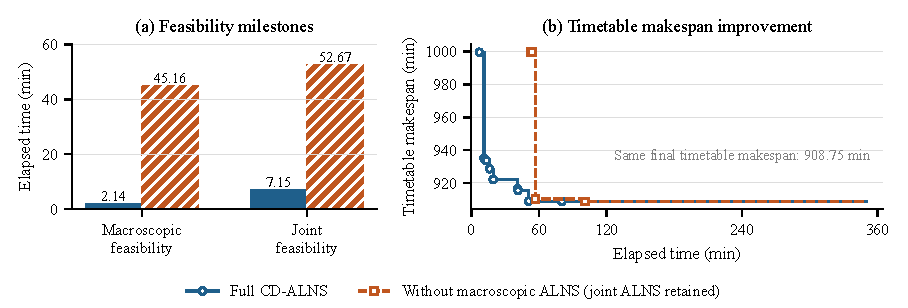
\includegraphics[width=\textwidth]{figures/fig6_ablation.pdf}
\caption{Effect of the macroscopic ALNS phase in the medium-scale case: (a) times to macroscopic and joint feasibility; (b) timetable makespan improvement. Both configurations attain the same timetable makespan of 908.75 min.}\label{fig:ablation}
\end{figure}

\subsection{Robustness over random seeds}\label{sec:seeds}
\begin{pending}[: E1, repeated runs]
Run CD-ALNS with 10 random seeds on each case (same time limits, hardware, and Gurobi version) and report, for $S$, $t_{\mathrm{feas}}$, and $t_{\mathrm{best}}$, the best, mean, worst, and standard deviation, and the number of runs that reach joint feasibility. Fill \cref{tab:seeds} and add box plots of $S$ and $t_{\mathrm{feas}}$.
\end{pending}
\begin{table}[htbp]
\centering\small
\caption{Results of CD-ALNS over 10 random seeds (to be completed).}\label{tab:seeds}
\begin{tabular}{@{}lccccccc@{}}\toprule
Case & Feasible runs & $S$ best & $S$ mean & $S$ worst & $S$ std. & $t_{\mathrm{feas}}$ mean & $t_{\mathrm{best}}$ mean\\\midrule
Small-scale & \tbd & \tbd & \tbd & \tbd & \tbd & \tbd & \tbd\\
Medium-scale & \tbd & \tbd & \tbd & \tbd & \tbd & \tbd & \tbd\\
Large-scale & \tbd & \tbd & \tbd & \tbd & \tbd & \tbd & \tbd\\\bottomrule
\end{tabular}
\end{table}

\subsection{Contribution of the algorithmic components}\label{sec:components}
\begin{pending}[: E2, component ablations and operator statistics]
On the medium- and large-scale cases (several seeds each), compare the full CD-ALNS with: (i) without J3 service frequency compensation; (ii) without J4 boundary extension; (iii) without J5 tight temporal links; (iv) uniform random operator selection instead of adaptive weights; (v) without fixed-structure re-optimization; (vi) a standard LNS with random destroy of trains and the same MILP repair. Report $S$, $t_{\mathrm{feas}}$, and $t_{\mathrm{best}}$ in \cref{tab:components}. In addition, report the selection frequency, success rate, and average time of each operator and scale per phase (from the iteration logs), e.g., as a heat map.
\end{pending}
\begin{table}[htbp]
\centering\small
\caption{Component ablations (to be completed; mean over seeds).}\label{tab:components}
\footnotesize\setlength{\tabcolsep}{4pt}
\begin{tabular}{@{}lcccccc@{}}\toprule
 & \multicolumn{3}{c}{Medium-scale} & \multicolumn{3}{c}{Large-scale}\\\cmidrule(lr){2-4}\cmidrule(l){5-7}
Configuration & $S$ & $t_{\mathrm{feas}}$ & $t_{\mathrm{best}}$ & $S$ & $t_{\mathrm{feas}}$ & $t_{\mathrm{best}}$\\\midrule
Full CD-ALNS & \tbd & \tbd & \tbd & \tbd & \tbd & \tbd\\
Without J3 (frequency compensation) & \tbd & \tbd & \tbd & \tbd & \tbd & \tbd\\
Without J4 (boundary) & \tbd & \tbd & \tbd & \tbd & \tbd & \tbd\\
Without J5 (tight temporal links) & \tbd & \tbd & \tbd & \tbd & \tbd & \tbd\\
Uniform operator selection & \tbd & \tbd & \tbd & \tbd & \tbd & \tbd\\
Without fixed-structure re-optimization & \tbd & \tbd & \tbd & \tbd & \tbd & \tbd\\
Standard LNS (random destroy, MILP repair) & \tbd & \tbd & \tbd & \tbd & \tbd & \tbd\\\bottomrule
\end{tabular}
\end{table}

\subsection{Value of integration}\label{sec:sequential}
\begin{pending}[: E3, sequential versus integrated planning]
Compare the integrated approach with a sequential approach that first optimizes stops and timetable at the macroscopic level (Phase 1 only, until the end of the time limit or optimality) and then solves station platforming for the fixed timetable (\cref{prop:decomp}), repairing remaining conflicts by retiming only (J2 with stops and orders fixed). Report the number of stations with unresolved conflicts after the second step, the resulting makespan, and the time to a jointly feasible timetable.
\end{pending}

\subsection{Scalability}\label{sec:scalability}
\begin{pending}[: E4, generated instance set]
Generate a family of instances from the medium-scale line by varying the number of trains (e.g., 30, 45, 60, 75, 90), the share of optional stops, and the tightness of the station service frequency rules (e.g., lower bounds scaled by 0.5, 1.0, 1.5). Run CD-ALNS (several seeds) and Direct MILP with the same time limit, and report success rates, makespans, times to feasibility, and, where available, solver bounds.
\end{pending}

\subsection{Sensitivity analysis}\label{sec:sensitivity}
\begin{pending}[: E5, operational parameters]
On the medium-scale case, vary one parameter at a time: lower bounds of the station service frequency rules, length of the maintenance windows, maximum running time supplement (e.g., 0\%, 2.5\%, 5\%, 7.5\% of the pure running time), the maximum number of overtakings per stop, and the waiting maximum dwell time. Report the effect on $S$, $P$, $R$, the number of stops, and the number of overtakings. These results support the managerial insights in \cref{sec:insights}.
\end{pending}

\subsection{Lower bounds}\label{sec:bounds}
\begin{pending}[: E6, optimality gaps (optional)]
Compute lower bounds on $S$ for the medium- and large-scale cases, e.g., from the macroscopic relaxation without platforming constraints, or from the LP relaxation of the full MILP, and report the resulting gaps of the CD-ALNS solutions.
\end{pending}

\section{Managerial insights}\label{sec:insights}
The experiments suggest several implications for railway planners.

\textbf{Macroscopic feasibility does not guarantee station feasibility.} In the medium-scale case, the macroscopically feasible timetable satisfied all section headways, which are lower bounds on the route headways, but still contained nine station conflicts (\cref{sec:convergence}). Using the most restrictive route headway at the macroscopic level would remove such conflicts, but it would also exclude timetables that are feasible with less restrictive routes. Planning tools that only check line capacity can therefore produce timetables that cannot be executed in busy stations, and a sequential approach may have to revise the timetable after platforming.

\textbf{Service frequency requirements shape the feasible stop changes.} In the best timetables, a large share of the station service frequency rules are binding (\cref{tab:solution}). In that situation, a planner who skips a stop to relieve a station must at the same time decide which other train stops in the same counting window, and whether that train can be accommodated on a track. The joint neighborhoods of the CD-ALNS make this trade-off explicit, which is also how timetable planners reason when adjusting a draft timetable manually.

\textbf{Compressing the operating period.} Minimizing the makespan accommodates all prescribed services in a shorter operating period, which leaves more of the day for maintenance or additional services. In the medium- and large-scale cases, the makespan of the first jointly feasible timetable was reduced by 5445~s and 3126~s, respectively, through coordinated changes in stops, orders, and station routings and through the joint re-optimization of all event times.

\textbf{Station resources.} The best timetables use only part of the available station tracks (\cref{tab:solution}); in the medium-scale case, 31 of the 63 tracks are used. Together with the critical activities of \cref{prop:longest}, this information indicates where additional capacity would or would not shorten the operating period.

\begin{pending}[: insights from E3--E5]
Add quantitative insights from the sensitivity analysis (\cref{sec:sensitivity}) and the comparison with sequential planning (\cref{sec:sequential}), e.g., the marginal effect of tighter service frequency rules or longer maintenance windows on the makespan, the value of allowing overtaking, and the makespan increase or feasibility loss of sequential planning.
\end{pending}

\section{Conclusions}\label{sec:concl}
This paper has studied the integrated train timetabling, stop planning, and platforming problem with the timetable makespan as the primary objective. We represented the problem on an event-activity network whose activities between trains are disjunctive and depend on the stopping and station routing decisions, and formulated it as a MILP with continuous event times. For a fixed structure of stops, orders, and station routings, the minimum makespan equals the length of a longest path in the selected network, and the station platforming problems decompose by station. Building on these properties, we developed a conflict-driven ALNS with nine destroy operators. Its joint neighborhoods couple the resolution of station conflicts with the coordinated changes to stops, arrival and departure times, and station routings that are needed to keep every affected service count within its bounds, and a restricted MILP repairs them while retaining all constraints that link free and fixed decisions.

In the computational experiments, CD-ALNS reaches the proven optimal makespan in the small-scale case. In the medium- and large-scale cases, it quickly finds jointly feasible timetables and further reduces their makespans, whereas direct MILP solution and an adapted LBBD find no jointly feasible timetable within six hours. In the paired medium-scale comparison, the macroscopic ALNS phase yields earlier joint feasibility and earlier attainment of the same final makespan, with worse secondary objectives. \tbd~\textit{Summarize here the results of the experiments E1--E5.}

Several directions remain for future research. First, lower bounds for the medium- and large-scale cases would allow the optimality gaps to be evaluated. Second, the approach could be extended to bidirectional lines with single-track sections and to network timetables with connections. Third, passenger-oriented objectives and robustness against delays could be added to the lexicographic objective, and the neighborhood construction could be combined with learning-based operator selection.

\section*{CRediT authorship contribution statement}
\tbd~\textit{To be completed by the authors, e.g.:} \textbf{Siyu Wu:} Conceptualization, Methodology, Software, Investigation, Writing -- original draft. \textbf{Lei Nie:} Supervision, Funding acquisition, Writing -- review \& editing. \textbf{Zhiyuan Yao:} \tbd. \textbf{Kewei Cao:} \tbd.

\section*{Declaration of competing interest}
The authors declare that they have no known competing financial interests or personal relationships that could have appeared to influence the work reported in this paper.

\section*{Data availability}
\tbd~\textit{To be completed by the authors (e.g., data will be made available on request, or a repository link).}

\section*{Declaration of generative AI and AI-assisted technologies in the writing process}
\tbd~\textit{To be completed by the authors in accordance with the Elsevier policy.}

\section*{Acknowledgements}
This research was supported by the National Natural Science Foundation of China (U2568220) and the China State Railway Group Co., Ltd. (P2026X001, P2024X002).


\bibliographystyle{elsarticle-harv}
\bibliography{refs}

\appendix
\section{Timetable of the large-scale case}\label{app:large}
\Cref{fig:large} shows the time--distance diagram of the best jointly feasible timetable of the large-scale case, with a makespan of 65\,849~s (1097.48~min).

\begin{figure}[htbp]
\centering
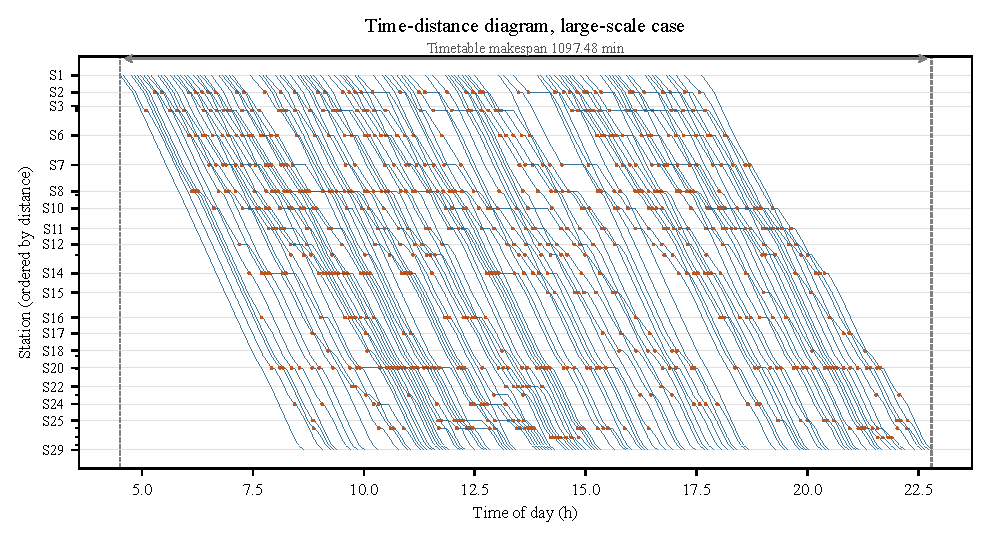
\includegraphics[width=\textwidth]{figures/fig_solution_large.pdf}
\caption{Time--distance diagram of the best jointly feasible timetable of the large-scale case; dots mark intermediate stops.}\label{fig:large}
\end{figure}

\end{document}
